\documentclass[a4paper,11pt,twoside]{report}
\title{Intermediate Language for JavaScript Final Report}




%%%%%%%%%%%%%%%%%%%%%%%%%%%%%%%%%%%%%%%%%%%%%%%%%%%%%%%%%%%%%%%%%%%%%%%%%%%%%

% Definitions for the title page
% Edit these to provide the correct information
% e.g. \newcommand{\reportauthor}{Timothy Kimber}

\newcommand{\reporttitle}{Intermediate Language for JavaScript}
\newcommand{\reportauthor}{Aubrianna Zhu}
\newcommand{\supervisor}{Philippa Gardner}
\newcommand{\degreetype}{Computing Science}

%%%%%%%%%%%%%%%%%%%%%%%%%%%%%%%%%%%%%%%%%%%%%%%%%%%%%%%%%%%%%%%%%%%%%%%%%%%%%

% load some definitions and default packages
%%%%%%%%%%%%%%%%%%%%%%%%%%%%%%%%%%%%%%%%%
% University Assignment Title Page 
% LaTeX Template
% Version 1.0 (27/12/12)
%
% This template has been downloaded from:
% http://www.LaTeXTemplates.com
%
% Original author:
% WikiBooks (http://en.wikibooks.org/wiki/LaTeX/Title_Creation)
%
% License:
% CC BY-NC-SA 3.0 (http://creativecommons.org/licenses/by-nc-sa/3.0/)
% 
%
%%%%%%%%%%%%%%%%%%%%%%%%%%%%%%%%%%%%%%%%%
%----------------------------------------------------------------------------------------
%	PACKAGES AND OTHER DOCUMENT CONFIGURATIONS
%----------------------------------------------------------------------------------------
%\usepackage[a4paper,hmargin=2.8cm,vmargin=2.0cm,includeheadfoot]{geometry}
\usepackage[left=2.5cm,right=2cm,top=2cm,bottom=2cm,includeheadfoot]{geometry}
\usepackage{textpos}
\usepackage{natbib} % for bibliography
\usepackage{tabularx,longtable,multirow,subfigure,caption}%hangcaption
\usepackage{fncylab} %formatting of labels
\usepackage{fancyhdr} % page layout
\usepackage{url} % URLs
\usepackage[english]{babel}
\usepackage{amsmath}
\usepackage{amssymb}
\usepackage{graphicx}
\usepackage{mathpartir}
\usepackage{listings}
\usepackage{dsfont}
\usepackage{epstopdf} % automatically replace .eps with .pdf in graphics
\usepackage{backref} % needed for citations
\usepackage{array}
\usepackage{latexsym}
\usepackage{changepage}
\usepackage{algorithm}
\usepackage{algorithmic}
\usepackage{multicol}
\usepackage{smartdiagram}
\usepackage[pdftex,pagebackref,hypertexnames=false,colorlinks]{hyperref} % provide links in pdf

\addtolength{\skip\footins}{11pt}

\newcommand{\myor}{\hspace{3pt}|\hspace{3pt}}

\lstdefinestyle{mystyle}{
    basicstyle=\footnotesize,
    breakatwhitespace=false,         
    breaklines=true,                 
    captionpos=b,                    
    keepspaces=true,                 
    numbers=left,                    
    numbersep=5pt,                  
    showspaces=false,                
    showstringspaces=false,
    showtabs=false,                  
    tabsize=2
}
 
\lstset{style=mystyle}

\hypersetup{pdftitle={},
  pdfsubject={}, 
  pdfauthor={},
  pdfkeywords={}, 
  pdfstartview=FitH,
  pdfpagemode={UseOutlines},% None, FullScreen, UseOutlines
  bookmarksnumbered=true, bookmarksopen=true, colorlinks,
    citecolor=black,%
    filecolor=black,%
    linkcolor=black,%
    urlcolor=black}

\usepackage[all]{hypcap}


%\usepackage{color}
%\usepackage[tight,ugly]{units}
%\usepackage{float}
%\usepackage{tcolorbox}
%\usepackage[colorinlistoftodos]{todonotes}
% \usepackage{ntheorem}
% \theoremstyle{break}
% \newtheorem{lemma}{Lemma}
% \newtheorem{theorem}{Theorem}
% \newtheorem{remark}{Remark}
% \newtheorem{definition}{Definition}
% \newtheorem{proof}{Proof}


%%% Default fonts
\renewcommand*{\rmdefault}{bch}
\renewcommand*{\ttdefault}{cmtt}



%%% Default settings (page layout)
%\setlength{\parindent}{0em}  % indentation of paragraph

\setlength{\headheight}{14.5pt}
\pagestyle{fancy}
\renewcommand{\chaptermark}[1]{\markboth{\chaptername\ \thechapter.\ #1}{}} 

\fancyfoot[ER,OL]{\sffamily\textbf{\thepage}}%Page no. in the left on odd pages and on right on even pages
\fancyfoot[OC,EC]{\sffamily }
\renewcommand{\headrulewidth}{0.1pt}
\renewcommand{\footrulewidth}{0.1pt}
\captionsetup{margin=10pt,font=small,labelfont=bf}


%--- chapter heading

\def\@makechapterhead#1{%
  \vspace*{10\p@}%
  {\parindent \z@ \raggedright \sffamily
    \interlinepenalty\@M
    \Huge\bfseries \thechapter \space\space #1\par\nobreak
    \vskip 30\p@
  }}

%---chapter heading for \chapter*  
\def\@makeschapterhead#1{%
  \vspace*{10\p@}%
  {\parindent \z@ \raggedright
    \sffamily
    \interlinepenalty\@M
    \Huge \bfseries  #1\par\nobreak
    \vskip 30\p@
  }}

\allowdisplaybreaks

% load some macros
% Here, you can define your own macros. Some examples are given below.

\newcommand{\R}[0]{\mathds{R}} % real numbers
\newcommand{\Z}[0]{\mathds{Z}} % integers
\newcommand{\N}[0]{\mathds{N}} % natural numbers
\newcommand{\C}[0]{\mathds{C}} % complex numbers
\renewcommand{\vec}[1]{{\boldsymbol{{#1}}}} % vector
\newcommand{\mat}[1]{{\boldsymbol{{#1}}}} % matrix


\date{\today}

\begin{document}

% load title page
% Last modification: 2015-08-17 (Marc Deisenroth)
\begin{titlepage}

\newcommand{\HRule}{\rule{\linewidth}{0.5mm}} % Defines a new command for the horizontal lines, change thickness here


%----------------------------------------------------------------------------------------
%	LOGO SECTION
%----------------------------------------------------------------------------------------


\includegraphics[width = 4cm]{imperial.pdf}\\[0.5cm] 

\center % Center remainder of the page

%----------------------------------------------------------------------------------------
%	HEADING SECTIONS
%----------------------------------------------------------------------------------------

\textsc{\Large Imperial College London}\\[0.5cm] 
\textsc{\large Department of Computing}\\[0.5cm] 

%----------------------------------------------------------------------------------------
%	TITLE SECTION
%----------------------------------------------------------------------------------------

\HRule \\[0.4cm]
{ \huge \bfseries \reporttitle}\\ % Title of your document
\HRule \\[1.5cm]
 
%----------------------------------------------------------------------------------------
%	AUTHOR SECTION
%----------------------------------------------------------------------------------------

\begin{minipage}{0.4\textwidth}
\begin{flushleft} \large
\emph{Author:}\\
\reportauthor
\end{flushleft}
\end{minipage}
~
\begin{minipage}{0.4\textwidth}
\begin{flushright} \large
\emph{Supervisor:} \\
\supervisor % Supervisor's Name
\end{flushright}
\end{minipage}\\[4cm]


%----------------------------------------------------------------------------------------
%	FOOTER & DATE SECTION
%----------------------------------------------------------------------------------------
\vfill % Fill the rest of the page with whitespace

\includegraphics[width=6cm]{imperial2.pdf}
\vspace{0.5cm}

Submitted in partial fulfillment of the requirements for the MSc degree in
\degreetype~of Imperial College London\\[0.5cm]

\makeatletter
\@date 
\makeatother


\end{titlepage}


% page numbering etc.
\pagenumbering{roman}
\clearpage{\pagestyle{empty}\cleardoublepage}
\setcounter{page}{1}
\pagestyle{fancy}

%%%%%%%%%%%%%%%%%%%%%%%%%%%%%%%%%%%%
\begin{abstract}
TODO
\end{abstract}

\cleardoublepage
%%%%%%%%%%%%%%%%%%%%%%%%%%%%%%%%%%%%
\section*{Acknowledgments}
TODO

\clearpage{\pagestyle{empty}\cleardoublepage}

%%%%%%%%%%%%%%%%%%%%%%%%%%%%%%%%%%%%
%--- table of contents
\fancyhead[RE,LO]{\sffamily {Table of Contents}}
\tableofcontents 


\clearpage{\pagestyle{empty}\cleardoublepage}
\pagenumbering{arabic}
\setcounter{page}{1}
\fancyhead[LE,RO]{\slshape \rightmark}
\fancyhead[LO,RE]{\slshape \leftmark}

%%%%%%%%%%%%%%%%%%%%%%%%%%%%%%%%%%%%
\chapter{Introduction}

\section{What is JavaScript}
JavaScript is the unofficial language of the Web---it is implemented in all major browsers, and its main purpose is to add interactivity to web pages by controlling both the style and the content of a browser's document object model. Increasingly, JavaScript is also being used on the server-side, as a means of interacting with databases. It exhibits a number of interesting features; for example, it supports prototypical inheritance rather than class inheritance, which is favored by many other programming languages. It allows for extensible objects---objects that can be altered after creation. Also, as there is virtually no difference between an object and a type, JavaScript does not have static typing or require type declarations~\cite{EcmaScript}. The intricacies of JavaScript will be discussed in chapter~\ref{sec:javascript}.

Since its inception, six versions of the standard have been developed, with the 6\textsuperscript{th} having been released in June 2015 \cite{international2015ecmascript}. This project will primarily target the 5\textsuperscript{th} edition of the ECMAScript standard, which was published in 2011. Significant changes have occurred in the 5\textsuperscript{th} edition, including the addition of accessor properties and a strict mode \cite{EcmaScript}, both of which will be addressed in this project.

\section{Verification and its Importance}
Computer scientists have created programming languages like JavaScript with the idea of instructing machines to perform actions in a human-like way, but possibilities for mistakes exist even in the creation phase. Indeed, a real life programming language was shown to have failed type safety five years after its creation \cite{drossopoulou1998towards}. It is of little help for correctness that, just like natural languages, programming languages evolve and become increasingly complicated. Moreover, programming language specifications are often written in plain prose that sometimes lacks detail or is simply ambiguous, which can result in diverging interpretations by different readers. When a programmer writes a piece of code that performs a certain task, without proper tools he cannot be entirely sure that his program will perform the task as required without side effects. In order to reduce errors and inconsistencies in different implementations of the same language, a formal verification system is necessary to prove that the programming languages are indeed performing correctly and as expected, with no ambiguity.

\section{JavaScript Verification}
Previous work on JavaScript verification that makes this project possible include formal reasoning about JavaScript using program logics \cite{Gardner:2012}; JSCert and JSRef, which are a mechanized specification of the ECMAScript standard and a certified reference interpreter, both written in the Coq proof assistant \cite{Bodin:2014}; and the JSIL intermediate language, which relies on JSCert and is at the core of this project. All of these works will be discussed in more detail in sections~\ref{sec:jslogic} to~\ref{sec:jsverify}.

\section{Outline of This Report}
After introducing programming language verification, this report will proceed to give an overview of the history and landscape of mechanized specifications for a variety of programming languages. Then, it will give a detailed explanation of operational semantics, a formalization method used by many mechanized verification projects, before providing more detail on the topic of JavaScript verification. Next, it will demonstrate existing work on translating ECMAScript standards into operational semantics, and from operational semantics to actual JSIL code. It will then provide detailed discussions on the topics of JavaScript, JSIL as an intermediate language, the JavaScript Array Library, and the Arguments Object, before moving on to discuss the process and results of testing the JSIL implementation. Lastly, a brief conclusion will wrap up the topics studied, and introduce possible future extensions. 

%%%%%%%%%%%%%%%%%%%%%%%%%%%%%%%%%%%%
\chapter{Background}
\section{History of Mechanized Specifications}\label{sec:hist}
There has been a long history of mechanized specification of programming languages. Initial formalizations were often simple, as they did not cover all aspects of the languages they targeted. Additionally, they tended to be non-executable and thus the appropriateness of their definitions were at times uncertain \cite{Ellison:2012}. Gradually, formalizations became increasingly mechanized, executable, and testable against standard test suites such as ECMAScript Test262 and GCC torture tests, or specific implementations such as Mozilla's JavaScript in order to ascertain real life correctness of these specifications. The following subsections will describe a number of mechanized specifications for various programming languages.

\subsection{ML}
\begin{description}
\item[Lee et al. 2007] This study created an internal language (IL), whose semantics is an explicitly-typed $\lambda$-calculus and follows a variation of the Harper and Stone\cite{Harper:2000} style, for standard ML \cite{Lee:2007}. This IL was able to capture all of the features in standard ML, and the proof of its type safety was successfully formalized in LF \cite{Harper:1993} and Twelf \cite{Pfenning98guide}.
\end{description}

\subsection{C}\label{sec:chist}
There has been many formal semantics written for C, ranging from those using abstract state machines \cite{Gurevich:1992}, to the HOL theorem proving system \cite{norrish:1998}, in addition to the two described below.
\begin{description}
\item[Leroy 2009] CompCert is a certified compiler from Clight to PowerPC assembly code, and it was designed to address the correctness of compilers, as most formal verification is done on source code rather than on code produced by optimized compilation. It used the Coq proof assistant for formal verification, to prove that the semantics of the generated assembly code corresponds exactly to the semantics of the source code \cite{Leroy-Compcert-CACM}. This verification is accomplished using eight intermediate languages from Clight to assembly, with each transformation having a formal proof that it preserves the semantics of the previous language in the translation chain.

\item[Ellison and Rosu 2012] This work employs $\mathbb{K}$ \cite{rosu-serbanuta-2010-jlap}, a semantic framework based on rewriting-logic, and Maude \cite{Clavel:2007}, a rewriting-logic engine that enables execution and analysis of the mechanized semantics \cite{Ellison:2012}. The $\mathbb{K}$-based semantics for C is executable and was tested against the GCC torture test suite \cite{Ellison:2012}. 
\end{description}

\subsection{Java}
As for C, there exists a large body of work concerning the formalization of Java. 
\begin{description}
\item[Drossopoulou and Eisenbach 1998] As early as 1998, a small step operational semantics has been defined for Java \cite{drossopoulou1998towards} \cite{Drossopoulou:1999} using a term rewrite system. This work has covered a substantial subset of the Java language, with a focus on proving that the type system indeed works correctly.

\item[Klein and Nipkow 2006] Another example is work done using the Isabelle theorem prover \cite{Paulson1989}, an environment to formalize and prove the type safety for Jinja \cite{KleinN-TOPLAS}, a variation of Java. The authors utilized both small step and big step operational semantics---the two styles are used in different aspects of the proof, but they are shown to be equivalent. This work is important because it was the first holistic formal analysis of a Java-like language, its virtual machine, and its compiler \cite{KleinN-TOPLAS}.

\item[Bogdanas and Rosu 2015] The most recent work done on formalizing Java follows the C example from section~\ref{sec:chist}, using $\mathbb{K}$ as the development tool for Java 1.4. In this project, all features in the Java specification were covered and tested \cite{Bogdanas:2015}, as $\mathbb{K}$ automatically provides the executable environment for the formal specification, named K-Java. 
\end{description}

\subsection{JavaScript}
This section presents four sample studies, with the first being a purely theoretical translation of the ECMAScript standard, whereas the other three also have executable portions.

\begin{description}
\item[Maffeis et al. 2008] The authors produced an extensive small step operational semantics for ECMAScript 3, encompassing about 70 pages of rules and definitions \cite{Maffeis:2008}. The main goal of this formalization was to analyze the security properties of JavaScript programs running in web browsers, as the operational semantics allowed the authors to understand what can and cannot interact with the heap when a program is run. This operational semantics was not directly executable, but the authors designed experiments to test certain constructs on different browser implementations, and found discrepancies between Firefox, Safari, and the JavaScript standard implementation \cite{Maffeis:2008}. This work was important in inspiring other researchers to pursue operational semantics as a way to fully understand JavaScript behavior.

\item[Politz et al. 2012] A formal semantics, S5, for the strict mode of ECMAScript 5.1 was developed following the semantics of $\lambda$\textsubscript{JS} \cite{Guha:2010}. It covers the core semantics of JavaScript, and all JavaScript features that are not immediately covered can be transformed via a desugaring function. It is executable and tested for conformance with the ECMAScript test suite, Test262. S5 focuses in particular, on the getters and setters (accessor properties), and the \texttt{eval} operator \cite{Politz:2012}.

\item[Bodin et al. 2014] In this work, the ECMAScript 5 standard was mechanized using pretty big step semantics (JSCert) and a reference interpreter (JSRef) was implemented using the Coq theorem prover. JSRef was proven correct with respect to JSCert, then extracted to OCaml using Coq's built-in extraction mechanism, and tested against Test262 \cite{Bodin:2014}. The correctness result ensures that both JSCert and JSRef are correct with respect to the JavaScript standard. The current project stems from this work, and JSCert and JSRef will be discussed in more detail in section~\ref{sec:jscert}.

\item[Park et al. 2015] Similar to the study presented in Section~\ref{sec:chist}, this formal semantics of JavaScript is also based on $\mathbb{K}$ \cite{k-primer-2013-v32}. KJS was tested against Test262, and its language construct closely resembles the ECMAScript standard. In addition, it was able to discover coverage deficiencies in Test262 itself \cite{Park:2015}.
\end{description}

\section{Operational Semantics}\label{sec:opsem}
Like natural languages, programming languages have the distinction between syntax and semantics. Syntax refers to the physical structure and rules of the language, defining valid variable names and correct placement of semicolons; semantics refers to the meaning of the program, specifying the actions and results of program commands. In regards to verification, semantics is what makes a program correct or incorrect. There are three different categories of program semantics: denotational, axiomatic, and operational. Operational semantics has turned out to be the category of choice, since it specifies meaning by giving the steps and behavior of a program during execution \cite{PittsAM:opespe}. In general, there are two ways of representing the semantics: small step and big step. 

Presented below is the syntax of a simple imperative programming language, whose syntax will be followed in the upcoming subsections. The $\mathtt{While}$ command will serve as a running example throughout this report.

$$
\arraycolsep=1.5pt
\begin{array}{rclcl}
B & \in & \mathrm{Bool} & ::= & \texttt{true} \myor \texttt{false} \myor E = E \myor E < E \myor B \& B \myor\neg B \myor \ldots \\
E & \in & \mathrm{Exp} & ::= & \texttt{x} \myor \texttt{n} \myor E + E \myor \ldots \\
C & \in & \mathrm{Com} & ::= & \texttt{x}:=E \myor \texttt{if B then C else C} \myor C; C \myor \texttt{skip} \myor \texttt{while B do C} \myor ...
\end{array}
$$

\noindent where we denote variables by $\texttt{x}$ and numbers by $\texttt{n}$. 
Configurations are defined as $\langle E,s \rangle$, $\langle B,s\rangle$ and $\langle C,s \rangle$, meaning expressions, booleans, and commands with respect to state $s$.

\subsection{Small Step}
Small step operational semantics is also called structural operational semantics, and it evaluates expressions one step at a time \cite{Lecture2}. Due to its fine granularity, small step semantics is often used to model type systems and concurrency \cite{chargueraud-13-pretty}, as well as mechanized programming language definitions. The relation between two states is represented by the $\rightarrow$ symbol, and an example of this semantics is given below. In S-LEFT, an expression is evaluated in the order from left to right, thus $\mathbf{E}_1$ is evaluated before $\mathbf{E}_2$. If the left hand side is already a numeral, then the expression on the right hand side, $\mathbf{E}$, will be evaluated in S-RIGHT. Once all expressions are evaluated, addition will occur as in S-ADD.
\begin{mathpar}
\inferrule[S-LEFT]{\mathbf{E}_1 \rightarrow \mathbf{E}'_1}{\mathbf{E}_1 + \mathbf{E}_2 \rightarrow \mathbf{E}'_1 + \mathbf{E}_2}
\and
\inferrule[S-RIGHT] {\mathbf{E} \rightarrow \mathbf{E}'}{n + \mathbf{E} \rightarrow n + \mathbf{E}'}
\and
\inferrule[S-ADD]{\underline{\texttt{n}_1} + \underline{\texttt{n}_2} = \underline{\texttt{n}_3}}{\texttt{n}_1 + \texttt{n}_2 \rightarrow \texttt{n}_3 }
\end{mathpar}

A more concrete example, $3 + ( 2 + 1 ) \rightarrow 3 + 3 \rightarrow 6$, would require the S-RIGHT rule to be applied to ( 2 + 1 ) and the S-ADD rule to produce 3 to give the intermediate stage 3 + 3, then another S-ADD to give the final result 6 \cite{Lecture2}.

As for a $\mathtt{While}$ command, only one rule is necessary as the semantics takes care of the recursive looping on its own. Only the initial step needs to be defined and the rule will carry on until it reaches a $\mathtt{skip}$ condition. Details for the small step evaluation rules for  sequential composition and conditionals have been omitted, but they both contribute towards defining the $\mathtt{While}$ semantics. The following small step semantics for $\mathtt{While}$ is presented in the Models of Computation course at Imperial for second-year Computing students. \footnote{It was necessary to self-study a portion of the materials presented in the second-year Models of Computation course to get up to speed with operational semantics.}

\begin{mathpar}
\inferrule[SS-WHILE]{ }{\langle \texttt{while B do C, s} \rangle \rightarrow_c \langle \texttt{if B then (C; while B do C) else skip, s} \rangle}
\end{mathpar}

\subsection{Big Step}
Big step operational semantics is also called natural operation semantics, and in contrast to small step, it evaluates the entire expression in one step and returns the final result immediately \cite{Lecture2}, and the behavior of one term can be seen as the composition of the behaviors of the sub-terms \cite{chargueraud-13-pretty}. The relation between two states is represented by the $\Downarrow$ symbol, and the same example is given below. In B-NUM, a number is evaluated to a number. The equivalent was not in the small step semantics because numbers are considered to be fully evaluated. In B-ADD, $\mathbf{E}_1$ and $\mathbf{E}_2$ are evaluated separately to two numbers, $\texttt{n}_1$ and $\texttt{n}_2$, respectively, while applying actual addition in the same rule to arrive at the final answer $\texttt{n}_3$.

\begin{mathpar}
\inferrule[B-NUM]{ }{\texttt{n} \Downarrow \texttt{n}}
\and
\inferrule[B-ADD] {\mathbf{E}_1 \Downarrow \texttt{n}_1 \\ \mathbf{E}_2 \Downarrow \texttt{n}_2 \\ \underline{\texttt{n}_1} + \underline{\texttt{n}_2} = \underline{\texttt{n}_3}}{\mathbf{E}_1 + \mathbf{E}_2 \Downarrow \texttt{n}_3}
\end{mathpar}

The same example yields $3 + ( 2 + 1 ) \Downarrow 6 $ for big step semantics because the final result is produced immediately \cite{Lecture2}. 

 The $\mathtt{While}$ command for big step semantics requires two different rules \cite{LectureBS}, one for when the boolean condition is $\mathtt{true}$, another for $\mathtt{false}$. In BS-WHILE-FALSE, the boolean condition \textit{B} evaluates to $\mathtt{false}$, so the command \textit{C} is never executed, and the program state \textit{s} stays the same after evaluation. In BS-WHILE-TRUE, \textit{B} evaluates to $\mathtt{true}$, so the while loop is unrolled once, command $C$ is executed, which alters the state from $s$ to $s'$, and the while loop is called recursively with the state $s'$.

\begin{mathpar}
\inferrule[BS-WHILE-FALSE]{\langle \texttt{B, s} \rangle \Downarrow \langle \texttt{false} \rangle}{\langle \texttt{while B do C, s} \rangle \Downarrow \langle \texttt{s} \rangle} \qquad
\inferrule[BS-WHILE-TRUE]{\langle \texttt{B, s} \rangle \Downarrow \langle \texttt{true} \rangle \quad \langle \texttt{C, s} \rangle \Downarrow \langle \texttt{s'} \rangle \quad \langle \texttt{while B do C, s'} \rangle \Downarrow \langle \texttt{s''} \rangle}{\langle \texttt{while B do C, s} \rangle \Downarrow \langle \texttt{s''} \rangle}
\end{mathpar} 

\subsection{Pretty Big Step}
A variation of big step semantics has been used in describing JavaScript program logic \cite{Bodin:2014} developed by Charguéraud \cite{chargueraud-13-pretty}. While big step semantics has the advantage of immediacy and hence intuitively makes more sense, it does have several disadvantages, the biggest of which is the redundancy of premises for many different evaluation rules when exceptions and/or divergence occur \cite{chargueraud-13-pretty}. Thus, for programs with no rule repetitions, big step semantics and pretty big step semantics can be quite indistinguishable, but if an entire programming language must be mechanized, big step semantics simply does not scale. Indeed, the work done so far with JavaScript verification follows the style of pretty big step semantics since it addresses the redundancy problem. The running example is given below. 

In $\mathbf{E}_1$ + $\mathbf{E}_2$, to avoid redundancy as in big step semantics, one expression is evaluated at a time and in the order from left to right. So PB-ADD evaluates the first expression, $\mathbf{E}_1$, and utilizes an operator $+_1$ for when the first expression is already evaluated. In PB-+\textsubscript{1}, the $+_1$ rule is defined by evaluating the second expression and utilizing a $+_2$ operator for when both expressions are numbers. PB-+\textsubscript{2} then performs the actual addition between two numbers using $+_2$, propagating the result of $+_2$ back to PB-+\textsubscript{1}, which then propagates its result to PB-ADD to yield the final result, and the cycle is complete. 
\begin{mathpar}
\inferrule[PB-ADD]{\mathbf{E}_1 \Downarrow \texttt{n}_1 \\ \texttt{n}_1 +_1 \mathbf{E} \Downarrow \texttt{n}}{\mathbf{E}_1 + \mathbf{E}_2 \Downarrow \texttt{n}}
\and
\inferrule[PB-+\textsubscript{1}] {\mathbf{E} \Downarrow \texttt{n}_2 \\ \texttt{n}_1 +_2 \texttt{n}_2 \Downarrow \texttt{n}_3}{\texttt{n} +_1 \mathbf{E} \Downarrow \texttt{n}_3}
\and
\inferrule[PB-+\textsubscript{2}] { }{\texttt{n}_1 +_2 \texttt{n}_2 \Downarrow \underline{\texttt{n}_1} + \underline{\texttt{n}_2}}
\end{mathpar}

This would also yield $3 + ( 2 + 1 ) \Downarrow 6$, but the difference here is that two different versions of the + operator were defined.

\section{JavaScript Specifications}

\subsection{JS Logic}\label{sec:jslogic}
Gardner et al. \cite{Gardner:2012} have demonstrated that a program logic based on separation logic can be used to reason about JavaScript, since separation logic is useful to reason about programs that manipulate the heap, and JavaScript stores the entire program state in the object heap. A concept of weak locality was employed to establish the soundness of reasoning, since program commands are required to be local but JavaScript commands are not \cite{Gardner:2012}. The actual soundness proof was done using big step operational semantics that was defined for most of the ECMAScript 3 standard. This big step  semantics supplements previous effort to develop a small step operational semantics for core ECMAScript 3 functionality by Maffeis et al. \cite{Maffeis:2008}. An explanation of operational semantics can be seen in Section~\ref{sec:opsem}.

\subsection{JSCert and JSRef}\label{sec:jscert}
JSCert is a Coq specification of JavaScript \cite{Bodin:2014}. JSCert rules are in the form of $t/S/C \Downarrow_s o$, where $t$ is a statement, $S$ is the object heap and environment record, $C$ is the execution context, and $o$ is the output, meaning that if we execute the statement $t$ starting from the object heap $S$ and execution context $C$, we will obtain the output $o$. The output consists of the final state of the heap and a completion triple indicating the type of the return, the type of return value, and the return label \cite{Bodin:2014}. JSCert can be used to reason only about the scenarios where the program terminates, and not those in which it diverges.

JSRef, on the other hand, although also written in Coq, is a reference interpreter rather than a specification. JSRef contains records of functions that evaluate various parts of JavaScript source code, and recursively returns the result of program execution \cite{Bodin:2014}. JSRef functions are extracted automatically into OCaml code thanks to Coq, which enables JSRef functions to be run directly on Test262 to establish the correctness of both JSRef and JSCert with respect to the ECMAScript standard.

\subsection{JSVerify}\label{sec:jsverify}
For languages such as C and Java, efforts to verify program correctness have well been underway, as described in Section~\ref{sec:hist}, yielding many integrated development environments (IDEs) that perform dynamic and static analyses of code and help programmers debug their programs. Current JavaScript IDEs provide little more than simple syntax highlighting and do not adequately address program correctness. Coupled with its dynamic nature, JavaScript code is often buggy \cite{Gardner:2012} and even vulnerable to security attacks \cite{Lee:2007}. 

The ideas presented in sections~\ref{sec:jslogic} and~\ref{sec:jscert} culminated into a verification project called JSVerify, which is currently ongoing. Its aims are to use separation logic to reason about JavaScript programs and provide proofs of their correctness. This project ties in with JSVerify in that JSVerify will actually analyze code written in the intermediate language JSIL from this project, in order to determine the corresponding JavaScript program's correctness. This can be accomplished because there exists a proof of correctness of the translation from JavaScript to JSIL.

\subsection{Intermediate Languages for JavaScript Verification}\label{sec:ir}
Most real world programming languages are far too complex for reasonable analysis, and simpler forms of these languages are necessary for verification. Intermediate representations provide that simplicity. Historically, intermediate representations have been used in compilers, translating the source language into an intermediate form before translating into assembly code \cite{Necula2002}. As the need for language verification arose, a form of intermediate representation, called intermediate language, found its usefulness in helping analyze the source program in addition to being used in compilers.

Currently, many intermediate languages exist, and one of the most prominent is that for C, called CIL. Unlike C, CIL has only one looping construct, it makes the return statement explicit for all functions, and it simplifies the type system \cite{Necula2002}.

\paragraph{JavaScript Intermediate Languages}
\begin{description}
\item[JSIR] One intermediate language is JSIR \cite{Livshits:2016:Misc}, which aims to make different analysis tools more unified and less platform-dependent. Much of its grammar is defined, and can be found in the Github as cited \cite{Livshits:2016:Misc}. However, up to this point, JSIR has not been implemented and there is no compilation provided from any higher-level programming language to JSIR.

\item[WALA] Another interesting intermediate language, initially developed by IBM, is WALA \cite{WALA}. Unlike most other intermediate languages which are developed and used in academia, WALA is a set of full-fledged Java libraries used in production code for static and dynamic analyses. Although the bytecode is written in Java, it also supports simple program analyses for JavaScript in the form of JS-WALA \cite{WALA2}.

\item[Lambda JS / S5] $\lambda$\textsubscript{JS} \cite{Guha:2010} is a small step operational semantics that claims to capture the essential features of JavaScript, except for the \texttt{eval} functionality. S5 extends $\lambda$\textsubscript{JS} to the ECMAScript 5 standard and it focuses on JavaScript's strict mode \cite{Politz:2012}. Additional features of S5 include accessors and covering the \texttt{eval} function. JavaScript is translated to the core $\lambda$\textsubscript{JS} language via a desugaring function, and both $\lambda$\textsubscript{JS} and $S5$ are executable and tested against a Mozilla test suite and the Test262 suite, respectively.

\item[JSIL] Like other intermediate languages, JSIL does not have many of the high-level language constructs. Instead, it has simple $\texttt{goto}$ commands with labels and actions that resemble assembly code. JSIL has a memory model that is similar to that of JavaScript, and since JavaScript heaps are paramount in determining the outcome of running programs, this similarity helps relate JSIL programs with JavaScript programs.\footnote{Active work is in progress for JSIL and pending publication.} As seen in the heap models below, JavaScript heaps map locations, $\mathcal{L}$, and JavaScript variables, $\mathcal{X}_{JS}$, to JavaScript values, $\mathcal{V}_{JS}$, and scope chains, $\mathcal{S}ch_{JS}$, whereas JSIL heaps map locations, $\mathcal{L}$, and JavaScript variables, $\mathcal{X}_{JS}$, to JSIL values, $\mathcal{V}_{JSIL}$.

\begin{center}
\begin{tabular}{p{9cm}} \hline
\textbf{JavaScript Heap Model} \\
$\texttt{h} \in \mathcal{H}_{JS} : \mathcal{L} \times \mathcal{X}_{JS} \rightharpoonup (\mathcal{V}_{JS} \cup \mathcal{S}ch_{JS})$  \\ \hline
\end{tabular}

\begin{tabular}{p{9cm}} \hline
\textbf{JSIL Heap Model} \\
$\texttt{h} \in \mathcal{H}_{JSIL} : \mathcal{L} \times \mathcal{X}_{JS} \rightharpoonup \mathcal{V}_{JSIL} $  \\ \hline
\end{tabular}
\end{center}

The syntax of JSIL will be discussed in detail in Chapter~\ref{sec:jsil}.

\item[High-Level Languages] Lastly, there are many studies focusing on high level constructs of JavaScript rather than using intermediate representations for JavaScript verification. For example, Jensen et al. \cite{unevalizer2012} describes a way to transform JavaScript programs to eliminate the use of \texttt{eval} functions to improve static analysis of JavaScript source code. But as these methods only verify the source programs, and not the programming language itself, they are outside the scope of this project and will not be discussed in further detail.
\end{description}

\section{Operational Semantics and Specification in Action}
\subsection{While Loop}
A simple $\mathtt{While}$ command in operational semantics was demonstrated for both small step and big step semantics in section~\ref{sec:opsem}. In JavaScript, however, the definition for $\mathtt{While}$ is much more complicated. The following subsections will describe the $\mathtt{While}$ command as defined in the JavaScript standard, in operational semantics, and finally in JSIL code.

\subsubsection{ECMAScript 5 Standard} 
The while statement is given as the following in chapter 12.6.2 \cite{EcmaScript}. Its definition makes use of various JavaScript constructs such as references, predefined JavaScript values, and label sets. It also depends on other built-in functions such as \texttt{ToBoolean} and \texttt{GetValue}. Thus to completely understand how $\mathtt{While}$ functions, one must understand these other constructs as well.

The production \textit{IterationStatement} : while \textit{( Expression ) Statement} is evaluated as follows:
\begin{enumerate}
\item Let \textit{V} = $\texttt{empty}$.
\item Repeat
\begin{enumerate}
\item[a.] Let \textit{exprRef} be the result of evaluating \textit{Expression}.
\item[b.] If ToBoolean(GetValue(\textit{exprRef})) is \textbf{false}, return ($\texttt{normal, \textit{V}, empty}$).
\item[c.] Let \textit{stmt} be the result of evaluating \textit{Statement}.
\item[d.]If \textit{stmt}.value is not $\texttt{empty}$, let \textit{V} = \textit{stmt}.value.
\item[e.]If \textit{stmt}.type is not $\texttt{continue}$ $||$ \textit{stmt}.target is not in the current label set, then
\begin{enumerate}
\item[i.] If \textit{stmt}.type is $\texttt{break}$ and \textit{stmt}.target is in the current label set, then
\begin{enumerate} 
\item Return ($\texttt{normal, \textit{V}, empty}$).
\end{enumerate}
\item[ii.] If \textit{stmt} is an abrupt completion, return \textit{stmt}.
\end{enumerate}
\end{enumerate}
\end{enumerate}

%\subsubsection{JSCert example for while semantics}
%??? unsure whether to include
%--> while semantics/operational rules
%e(Pjs) = Pjsil with Pjsil (compilation of actual construcst, rewriting

%COMPILING:
%x :=e:
%REWRITING
% 	e(e) = cmd, xe
%RUNTIME FUNCTIONS
%	cmd
%    x1 := getValue(xe)
%    x2 := refv(lg, "x")
%    xpv := putvalue(x2, x1)
%    all can throw errorws 

\subsubsection{ES5 Strict Operational Semantics} 
Based on the ECMAScript standard definition, operational semantics for the $\mathtt{While}$ command in JSIL is much more complicated since it needs to faithfully represent the standard. Each bullet in the standard's text is transcribed into a rule in the operational semantics, and the repeat statement is taken care of by loop unrolling of the semantics.

In the style of pretty big step semantics, the relation takes the form of $L, l \vdash \langle h, s \rangle \Downarrow \langle h', o \rangle$. $L$ is the scope chain, $l$ is the location of \textit{this}, $h$ and $h'$ are the initial and final heaps, $s$ is the statement to be evaluated, and $o$ is the outcome. In the rules below, $s$ is defined to be $while(e){s}$, and $\Downarrow^\gamma$ represents the actual evaluation of expressions or statements. 

\begin{mathpar}
\inferrule[While]{L, l \vdash \langle h, \textnormal{while}_1(e) \{ s, \textnormal{empty} \} \rangle \Downarrow \langle h', o' \rangle}{L, l \vdash \langle h, \textnormal{while}(e) \{ s \} \rangle \Downarrow \langle h', o' \rangle}
\and
\inferrule[While-1] {L, l \vdash \langle h, e \rangle \Downarrow^\gamma \langle h_1, o_1 \rangle \\\\ L, l \vdash \langle h_1, \textnormal{while}_2(o_1,e) \{ s,o \} \rangle \Downarrow \langle h_2, o_2 \rangle}{L, l \vdash \langle h, \textnormal{while}_1(e) \{ s,o \} \rangle \Downarrow \langle h_2, o_2 \rangle}
\and
\inferrule[While-2(true)]{\neg \textnormal{False}(v) \\ L, l \vdash \langle h, s \rangle \Downarrow^\gamma \langle h_1, o_1 \rangle \\\\ L, l \vdash \langle h, \textnormal{while}_3(e) \{ s,o,o_1 \} \rangle \Downarrow \langle h_2, o_2 \rangle}{L, l \vdash \langle h, \textnormal{while}_2(v,e) \{ s,o \} \rangle \Downarrow \langle h_2, o_2 \rangle}
\and
\inferrule[While-2(false)]{\textnormal{False}(v)}{L, l \vdash \langle h, \textnormal{while}_2(v,e) \{ s, o \} \rangle \Downarrow \langle h, o \rangle}
\and
\inferrule[While-3(value)]{L, l \vdash \langle h, \textnormal{while}_1(e) \{ s, v \} \rangle \Downarrow \langle h_1, o_1 \rangle}{L, l \vdash \langle h, \textnormal{while}_3(e) \{ s, o,v \} \rangle \Downarrow \langle h_1, o_1 \rangle}
\and
\inferrule[While-3(return)]{L, l \vdash \langle h, \textnormal{while}_3(e) \{ s,o, \textnormal{ret}\ v \} \rangle \Downarrow \langle h, \textnormal{ret}\ v \rangle}{}
\and
\inferrule[While-3(empty)]{L, l \vdash \langle h, \textnormal{while}_1(e) \{ s,o \} \rangle \Downarrow \langle h_1, o_1 \rangle}{L, l \vdash \langle h, \textnormal{while}_3(e) \{ s, o,\textnormal{empty} \} \rangle \Downarrow \langle h_1, o_1 \rangle}
\end{mathpar}

\subsubsection{JSIL Code}
Compared to the JSIL operational semantics, there are a few constructs here not represented above, such as the \textit{fresh}() command, which creates a fresh JSIL variable to hold a return value. 

The \texttt{::} symbol represents concatenation of commands, and the \texttt{goto} command  has two different forms---\texttt{goto} \textit{i} directs the flow of control directly to line \textit{i}, and \texttt{goto} [e] \textit{i, j} first evaluates e, and if the evaluation result is \texttt{true}, the flow of control will go to line \textit{i}, otherwise to line \textit{j}. The \texttt{+} and \texttt{-} notations in the \texttt{goto} commands represent whether the program flow should go down or go up a certain number of lines, respectively, and the \texttt{\#} notation represents the number of lines that a certain command occupies, so $+\#cl_s$ means to go down the program the number of lines in $cl_s$. The JSIL program terminates when it reaches a \texttt{skip} command.
\begin{center}
\begin{minipage}{10cm}
\begin{lstlisting}[escapeinside={(*}{*)}]
(*$\textbf{let}\ x_e = fresh();\ x_s = fresh();$*)
    (*$cl_e = \mathcal{C}_m(e, x_e);\ cl'_e = \mathcal{W}_{\gamma} (x_e);$*)
    (*$cl_s = \mathcal{C}_m(s, x_s);\ cl'_s = \mathcal{W}_{\gamma}(x_s);$*)
    (*$e = (x_e = \textnormal{false})\ ||\ (x_e = \textnormal{undefined})\ ||\ (x_e = \textnormal{null})\ ||\ (x_e = "")$*)
    (*$\textbf{in} $*)
        (*$x := \textnormal{empty}$*)
        (*$cl_e :: cl'_e$*)
        (*$\texttt{goto}\ [e]\ [+\#cl_s +\#cl'_s +4], [+1]$*)
        (*$cl_s :: cl'_s$*)
        (*$\texttt{goto}\ [x_s\ != \textnormal{empty}]\ [+1], [+2]$*)
        (*$x := X_s$*)
        (*$\texttt{goto}\ [-\#cl_e -\#cl'_e -\#cl_s -\#cl'_s -3]$*)
        (*$\texttt{skip}$*)
\end{lstlisting}
\end{minipage}
\end{center}

\subsection{Internal JavaScript Function: Get}\label{sec:get}
An example of a JavaScript internal function that the $\mathtt{While}$ command uses is [[Get]], because during execution of $\mathtt{While}$, variables must be dereferenced to obtain their values. Indeed, the \textit{GetValue} command mentioned in step 2.b of $\mathtt{While}$ makes use of [[Get]] in its definition. [[Get]] itself depends on another internal function [[GetProperty]], which returns the property descriptor of the named property of this object or undefined \cite{EcmaScript}. This section follows the structure of the previous section, first describing the JavaScript standard, then the JSIL operational semantics, and finally JSIL code.

\subsubsection{ECMAScript 5 Standard}\label{sec:getstandard}
When the [[Get]] internal method of \textit{O} is called with property name \textit{P}, the following steps are taken:
\begin{enumerate}
\item Let \textit{desc} be the result of calling the [[GetProperty]] internal method of \textit{O} with property name \textit{P}.
\item If \textit{desc} is \textbf{undefined}, return \textbf{undefined}.
\item If IsDataDescriptor(\textit{desc}) is \textbf{true}, return \textit{desc}.[[Value]].
\item Otherwise, IsAccessorDescriptor(\textit{desc}) must be true so, let \textit{getter} be \textit{desc}.[[Get]].
\item If \textit{getter} is \textbf{undefined}, return \textbf{undefined}.
\item Return the result calling the [[Call]] internal method of \textit{getter} providing \textit{O} as the \textbf{this} value and providing no arguments.
\end{enumerate}

\subsubsection{ES5 Strict Operational Semantics}
The formalization of [[Get]] also closely follows the ECMAScript standard. Here \textsubscript{g} refers to [[Get]] and \textsubscript{gp} refers to [[GetProperty]]. In G-getProp, the result of calling [[GetProperty]] with $x$ is stored as $o$, which is then used as the input for [[Get]]. In G-propUndef, if the input for [[Get]] is undefined, then the returned result will be undefined. In G-propDefData, $d$ is a data descriptor, and the return value $v$ is the \textit{Value} attribute of $d$. in G-propDefAccGetUndef, $d$ is an accessor descriptor, and $d$'s \textit{Getter} attribute is undefined, so undefined is returned. And lastly in G-propDefAccGetDef, $d$ is an accessor descriptor, its \textit{Getter} attribute is defined and assigned as $a_g$, and $a_g$ is called to return the final outcome $o_f$.

\begin{mathpar}
\inferrule[G-getProp]{L, v_t \vdash \langle h, \mathcal{I}^o_{gp}(x) \rangle \Downarrow \langle h, o \rangle \\\\ L, v_t \vdash \langle h, \mathcal{I}^o_g(o)_1 \rangle \Downarrow \langle h_f, o_f \rangle}{L, v_t \vdash \langle h, \mathcal{I}^o_g(x) \rangle \Downarrow \langle h_f, o_f \rangle}
\and
\inferrule[G-propUndef] {L, v_t \vdash \langle h, \mathcal{I}^o_g(\textnormal{desc undefined}_1) \rangle \Downarrow \langle h, \textnormal{desc undefined} \rangle}{}
\and
\inferrule[G-propDefData]{\mathcal{P}_{(dd)}(d) \\ v=d.[[V]]}{L, v_t \vdash \langle h, \mathcal{I}^o_g(\textnormal{desc}\ d)_1 \rangle \Downarrow \langle h, v \rangle}
\and
\inferrule[G-propDefAccGetUndef]{\mathcal{P}_{(ad)}(d) \\ d.[[G]]=\textnormal{undefined}}{L, v_t \vdash \langle h, \mathcal{I}^o_g(\textnormal{desc}\ d)_1 \rangle \Downarrow \langle h, \textnormal{undefined} \rangle}
\and
\inferrule[G-propDefAccGetDef]{\mathcal{P}_{(ad)}(d) \\ a_g = d.[[G]] \neq \textnormal{undefined} \\ L, v_t \vdash \langle h, a_g() \rangle \Downarrow \langle h_f, o_f \rangle}{L, v_t \vdash \langle h, \mathcal{I}^o_g(\textnormal{desc}\ d)_1 \rangle \Downarrow \langle h_f, o_f \rangle}
\end{mathpar}

\subsubsection{JSIL Code}
The JSIL translation faithfully follows the ECMAScript standard. The procedure \textit{o}\_\_\textit{get} takes two parameters, the object itself and a property name. The [[GetProperty]] internal function is first located, then called. Since the property name may not exist, [[GetProperty]] is called with an error label, \textit{elab}, to throw errors as necessary. Depending on whether [[GetProperty]] has returned undefined, \textit{o}\_\_\textit{get} either returns or determines the descriptor type of the result. Descriptors are modeled as a list of elements, with the zeroth element being a character that signals the type of the descriptor. For instance, data descriptors have `d' as the first element, accessor descriptors have `a', and general descriptors have `g'. For data descriptors, the first element is the \textit{Value} attribute, and for accessor descriptors, it is the \textit{Getter} attribute. The \texttt{nth} function indexes the n\textsuperscript{th} element in a list. If the descriptor is a data descriptor, its value is returned; if it is an accessor descriptor and its \textit{Getter} is undefined, undefined is returned. Otherwise, the program will find the scope of the descriptor's \textit{Getter}, and the location of the \textit{Getter}'s [[Call]] method, before actually calling the \textit{Getter} function and returning.

\begin{center}
\begin{minipage}{9cm}
\begin{lstlisting}
proc o__get (l, prop) {
			gp := [l, ``@getProperty"];
			xret := gp (l, prop) with elab;	
			goto [xret = $$undefined] rlab def;
			
	def:	d := nth (xret, 0);
			xret := nth (xret, 1);
			goto [d = "d"] rlab acc;
			
	acc:	goto [xret = $$undefined] rlab get;
	get:	xsc := [xret, ``@scope"];
			fun := [xret, ``@call"];
			xret := fun (xsc, l) with elab;
			
	rlab:	skip;
	elab:	skip
}
with
{
    ret: xret, rlab;
    err: xret, elab;
};
\end{lstlisting}
\end{minipage}
\end{center}

\chapter{This Project and Concurrent Progress}
%%TODO%%
%%%%%%%%%%%%%%%%CHAPTER NEEDS TO BE UPDATED%%%%%%%%%%%%%%%%%%
Previous work has already been done on JSIL and the compiler, and this project seeks to expand JSIL to include descriptors, arguments object, and other library functions. Concurrently, tests against ECMAScript Test262 will be run to prove correctness for the implementation. For example, the memory model for both JavaScript and JSIL representations has already been changed to incorporate JavaScript descriptors, $\mathcal{D}_{JS}$, and the new JavaScript heap model will look like below, rather than the one presented in section~\ref{sec:ir}.

\begin{center}
\begin{tabular}{p{9cm}} \hline
\textbf{JavaScript Heap Model} \\
$\texttt{h} \in \mathcal{H}_{JS} : \mathcal{L} \times \mathcal{X}_{JS} \rightharpoonup (\mathcal{V}_{JS} \cup \mathcal{S}ch_{JS} \cup \mathcal{D}_{JS})$  \\ \hline
\end{tabular}

\begin{tabular}{p{9cm}} \hline
\textbf{JSIL Heap Model} \\
$\texttt{h} \in \mathcal{H}_{JSIL} : \mathcal{L} \times \mathcal{S}tr \rightharpoonup \mathcal{V}_{JSIL}  $  \\ \hline
\end{tabular}
\end{center}

\section{ES5 Strict and Core ES5 Strict}\label{sec:strict}
Strict mode was a concept introduced in the fifth version of the ECMAScript standard \cite{EcmaScript}, and it presents slightly different semantics compared to the non-strict version in the following significant ways: in strict mode, the only object environment record is the global object, variables cannot get assignment without first being declared, and errors will always be thrown when needed. The scope of strict mode is within the specific code unit that imposes strict mode, so a JavaScript program could possibly include both strict and non-strict code components \cite{EcmaScript}.

Strict mode influences the implementation of the language in multiple ways. One example would be in resolving the naming reference of variables. An abstract operation, IsStrictReference(V) (V is a Reference), returns the strict reference component of V \cite{EcmaScript}, and it is used in internal functions such as [[getValue]] and [[putValue]], like the [[Get]] internal function discussed in section~\ref{sec:get}.

The initial phase of this project seeks to complete the implementation of core strict mode, with core defined as the native language constructs and library functions that tap into these constructs. All other library functions that could be defined using what is already in core are not included in this initial stage but will be incorporated later on in the project.

\section{Contrast JSIL Without and With Descriptors}
Work by my supervisors to improve JSIL has been concurrently underway since I started this project, and most notably is the recent inclusion of descriptors into the memory model.

The following code snippets demonstrate the difference that descriptors can make in JSIL. On the left is JSIL code for [[Get]] without descriptors, and which will be referred to as \textit{LHS-without}, and on the right, JSIL with descriptors as presented before, and will be referred to as \textit{RHS-with}. Many internal functions make use of descriptors, thus without which the JSIL representation of JavaScript would simply be incorrect.

\begin{minipage}{.45\textwidth}
\begin{lstlisting}
proc o__get(l, prop) {
          gp := [l, "@getProperty"];
    rlab: xret := gp (l, prop);
}
with
{
    ret: xret, rlab;
}
\end{lstlisting}
\end{minipage}%
\hfill
\begin{minipage}{.50\textwidth}
\begin{lstlisting}
proc o__get (l, prop) {
			gp := [l, "@getProperty"];
			xret := gp (l, prop) with elab;	
			goto [xret = $$undefined] rlab def;
			
	def:	d := nth (xret, 0);
			xret := nth (xret, 1);
			goto [d = "d"] rlab acc;
			
	acc:	goto [xret = $$undefined] rlab get;
	get:	xsc := [xret, "@scope"];
			fun := [xret, "@call"];
			xret := fun (xsc, l) with elab;
			
	rlab:	skip;
	elab:	skip
}
with
{
    ret: xret, rlab;
    err: xret, elab;
};
\end{lstlisting}
\end{minipage}

Recall section~\ref{sec:getstandard} presented the ECMAScript standard for the [[Get]] internal function. The JSIL implementation without descriptors is much shorter because all the steps in the standard that deal with descriptors are inapplicable. Starting from step 3 which states "If IsDataDescriptor(\textit{desc}) is \textbf{true}, return \textit{desc}.[[Value]]", \textit{LHS-without} simply cannot address the concept of descriptors, whereas \textit{RHS-with} implements step 3 in the \textit{def} code block. The three subsequent steps, "Otherwise, IsAccessorDescriptor(\textit{desc}) must be true so, let \textit{getter} be \textit{desc}.[[Get]]", "If \textit{getter} is \textbf{undefined}, return \textbf{undefined}", and "Return the result calling the [[Call]] internal method of \textit{getter} providing \textit{O} as the \textbf{this} value and providing no arguments" also went unaddressed in \textit{LHS-without}, but were implemented as the \textit{acc} and \textit{get} code blocks in \textit{RHS-with}.

\section{Scope and Aims}
This project aims to complete the Object.prototype and Array libraries in their JSIL implementation. The Object.prototype library encompasses seven built-in functions for a total of two pages in the ECMAScript standard, while the Array library includes 28 built-in functions for a total of 20 pages. All of the functions in these libraries will be implemented on the JSIL level, and tested against the standard test suite, Test262, on a continually integrated basis. 

Another topic of interest is the arguments object, which is initially described in section 10.6 and mentioned throughout section 15. Implementing the arguments object entails altering the compiler that translates ES5 strict code into JSIL, as well as testing against Test262 to ensure the correctness of the compiler.

\section{Testing}
%%TODO%%
%need to figure out exact numbers for each test case category
The current testing framework includes the entire ECMAScript 6 test suite (ES6 Test262) which consists of 14998 test cases. Previous testing has applied several rounds of filtering to discard irrelevant test cases, including ES6-only features, non-strict functionality, non-core functionality, and so on, after which 4599 tests remain. Of these 4599, current implementation of JSIL covers 2388 test cases, and the rest of the 2211 tests need to be worked on. The exact number of test cases that this project will cover remains to be defined.

The interactive testing framework is available online from inside the Imperial network, but soon it will be integrated into a publicly accessible web address and will become continuously integrated into the JSIL project. At that point, each JSIL commit can be viewed from the testing portal, and the results can be compared with previous commits to determine whether the commit improved or worsened test coverage. Thus, JSIL development and testing will be done concurrently, and mistakes will be spotted and addressed as soon as they appear.

%%%%%%%%%%%%%%%%%%%%%%%%%%%%%%%%%%%%
\chapter{JavaScript}\label{sec:javascript}
\section{Definition of Objects}
JavaScript is a language that relies heavily and primarily on Objects, which are collections of \textbf{properties}, each with zero or more \textbf{attributes} that define the property \cite{EcmaScript}. Properties can hold the following types: Objects, primitive values, or functions, which are a type of special Objects. The JavaScript values and additional boolean values associated with each property are the attributes of the property. Each attribute has its own name and value. Essentially, properties can be seen as name-value pairs, with the names generally being primitive strings, and the values being one of the three types previously mentioned. Objects can be created via literal notation or via Object constructors that create and initialize the Objects, and then establishes the prototype chain for the Object \cite{EcmaScript}. Within an object, there are two types of properties - own properties and inherited properties. Own properties are those defined within the current object, and inherited properties are those defined in the object's prototype chain.

Unlike Objects in most other programming languages such as C++ and Java, JavaScript Objects are dynamic, which means they can be altered after creation. For example, a Person class is defined in Java below. This class has two properties - a String variable for the person's name, and an integer variable for the person's age. A Person Object called \textit{bob} is created in the main method on line 11, initialized with a name String as "Bob", and an age of 30 years old. If \textit{bob} has a birthday, then his age can be changed by providing a different value to the \textit{bob.age} variable. But in case we wanted to add another property, gender, to specify that \textit{bob} is male, then the code on line 13 would produce an error saying \textit{bob.gender} cannot be resolved. Since \textit{gender} is not included in the class declaration, any Object of Person class cannot possibly have a \textit{gender} property.

\begin{adjustwidth}{4cm}{4cm}
\begin{lstlisting}
public class Person {
    private String name;
    private int age;
    
    public Person(String n, int a) {
        name = n;
        age = a;
    }
    
    public static void main(String[] args) {
        Person bob = new Person("Bob", 30);
        bob.age = 31;
        bob.gender = "male";
    }
}
\end{lstlisting}
\end{adjustwidth}

Below defines a Person class in JavaScript, intentionally using similar syntax as the Java code above for comparison. The \textit{alice} Object is created on line 8 with a name String as "Alice", and an age of 35 years old. When \textit{alice} celebrates her birthday, her age can be altered using dot notation similar to that of \textit{bob}. When we want to specify the gender of \textit{alice} however, using code on line 10, JavaScript would throw no error and simply change the \textit{alice} Object as required.
\begin{adjustwidth}{4cm}{4cm}
\begin{lstlisting}
class Person {
	constructor(n, a) {
		this.name = n;
		this.age = a;
	}
}

var alice = new Person("Alice", 35);
alice.age = 36;
alice.gender = "female";
\end{lstlisting}
\end{adjustwidth}

It is easy to see why this would make JavaScript code much more complicated and error-prone. If the programmer accidentally makes changes to an Object in this manner, no error message will alert him or her of this, and hence a verification tool would come in extremely handy.

\section{Properties}
There are two types of properties in JavaScript - named properties and internal properties \cite{EcmaScript}. Named properties, by definition, associate user-defined name strings with JavaScript descriptors, whereas internal properties do not have user-defined names. Named properties can either be data properties or accessor properties. Data properties associate a name with a JavaScript value, plus a set of boolean values that specify additional information about the property. These boolean values will be explained in further detail in section~\ref{sec:attributes}. Accessor properties associate a name with two JavaScript functions, a getter and a setter, in addition to a similar set of boolean values. The getter and setter are used to retrieve or store, respectively, the JavaScript value associated with the property. All objects share a set of twelve internal properties that get defined when the objects are created, including the Object's prototype, class, and so on. There are an additional twelve internal properties that only apply to certain types of Objects, for example, Function Objects alone have the [[Call]] internal method.

\subsection{Attributes}\label{sec:attributes}
Both categories of named JavaScript properties have attributes that serve to describe the state of the property. Data properties and accessor properties share two of these attributes, [[Enumerable]] and [[Configurable]], while they differ in the other two. Data properties have the [[Value]] and [[Writable]] attributes, while accessor properties have [[Get]] and [[Set]].

\begin{description}
\item[Value] The [[Value]] attribute can take on any of the ECMAScript types, and it represents what is intuitively the value of the property. Valid types are listed below, and the default value is Undefined.
\begin{multicols}{2}
\begin{itemize}
	\item Undefined
	\item Null
	\item Boolean
	\item String
	\item Number
	\item Object
	\item Reference Specification
	\item List Specification
	\item Completion Specification
	\item Lexical Environment Specification
	\item Environment Record Specification
\end{itemize}
\end{multicols}

\item[Writable] The [[Writable]] attribute is a Boolean value, and it describes whether this property's [[Value]] attribute can be altered using the [[Put]] internal method. The default value is False.

\item[Get] The [[Get]] attribute can be of the Function Object type, but the default value is Undefined. When the property's getter is invoked, the [[Call]] internal method of the Function Object is called with no arguments in order to return the property's value.

\item[Set] The [[Set]] attribute can be of the Function Object type, but the default value is Undefined. When the property's setter is invoked, the [[Call]] internal method of the Function Object is called with an appropriate assignment value for the property. This setter function call may or may not alter the result of the getter function call, since the setter is not required to set the same variable as the getter retrieves.

\item[Enumerable] The [[Enumerable]] attribute is a Boolean value. If True, the property will be used in for-in enumeration. The default value is False.

\item[Configurable] The [[Configurable]] attribute is a Boolean value, and it describes whether the property can be deleted, whether the property's attributes can be altered, and whether a data property can be changed into an accessor property and vice versa. The default value is False.
\end{description}

\subsection{Descriptors}
Descriptors are a JavaScript language construct used to describe named property attributes, so that programs can access and manipulate the attributes as necessary. Descriptors are represented as name-value pairs, similar to Objects in a way, except the only valid names are the named property attribute names, and the values are the corresponding attribute values. Thus, descriptors can either be data descriptors or accessor descriptors, determined by the following two abstract operations.

\begin{description}
\item[IsDataDescriptor(Desc)] Returns False if Desc is Undefined, and returns True if both the [[Value]] and [[Writable]] fields are present.

\item[IsAccessorDescriptor(Desc)] Returns False if Desc is Undefined, and returns True if both the [[Get]] and [[Set]] fields are present.
\end{description}

In case that a descriptor is defined, but is neither a data descriptor nor an accessor descriptor, then it is a generic descriptor. Because of the similarity in structure between descriptors and Objects, the two can be interchanged using the following abstract operations.

\begin{description}
\item[FromPropertyDescriptor(Desc)] This operation takes a descriptor, Desc, and converts it into an Object with four properties. If Desc is a data descriptor, the new Object will have two properties named "value" and "writable", and if Desc is an accessor descriptor, the new Object will have two properties named "get" and "set". The new Object will also have the "enumerable" and "configurable" properties. Each new property will be represented by a new data descriptor with the [[Value]] attribute being the descriptor's original value field, and the Boolean value True for the [[Writable]], [[Enumerable]], and [[Configurable]] attributes.

\item[ToPropertyDescriptor(Obj)] This operation takes an Object, Obj, and converts it into a descriptor by calling the [[HasProperty]] internal method, described in the next section, on each of these String values: "enumerable", "configurable", "value", "writable", "get", "set". If Obj has properties with the same names as these Strings, then the corresponding descriptor field is populated with the value returned by the [[Get]] internal method of Obj with the String as input. If Obj has property names that correspond to both data descriptor and accessor descriptor field names, the conversion operation is considered illegal.
\end{description}

\subsection{Internal Properties}
Internal properties describe additional inherent information about Objects, and they cannot be directly accessed by the programmer. The following internal properties hold one or multiple particular types of JavaScript values, and their values can be modified through implementation-specific helper functions.

\begin{description}
\item[Prototype] The [[Prototype]] property can be of Object type or Null, and it represents the prototype for the current Object. This property is accessed in the prototype chain to determine inheritance behavior. The prototype chain of any Object must be of finite length. 

\item[Class] The [[Class]] property is a String value that specifies the classification of the current Object. The value of [[Class]] for built-in JavaScript Objects are the following.
\begin{multicols}{3}
\begin{itemize}
	\item "Arguments"
	\item "Array"
	\item "Boolean"
	\item "Date"
	\item "Error"
	\item "Function"
	\item "JSON"
	\item "Math"
	\item "Number"
	\item "Object"
	\item "RegExp"
	\item "String"
\end{itemize}
\end{multicols}

\item[Extensible] The [[Extensible]] property is a Boolean value that indicates whether additional named own properties can be added to the current Object, and once it has been changed to False, it cannot be changed back to True. If the value is False, the values for [[Prototype]] and [[Class]] of the current Object also can no longer be altered. A JavaScript Object would behave more closely to a class-based Object if its [[Extensible]] property is False.
\end{description}

The following internal properties represent internal methods of the same name, consisting of predefined procedures that operate on the Object in some manner.
\begin{description}
\item[GetOwnProperty] The [[GetOwnProperty]] internal method takes a property name as input, and returns the descriptor corresponding to the property name if it exists in the Object itself, and returns Undefined if it does not exist.

\item[GetProperty] The [[GetProperty]] internal method takes a property name as input, and returns the descriptor corresponding to the property name if it exists at any stage within the Object's prototype chain, and returns Undefined if it does not exist. [[GetProperty]] is recursively defined - it first calls the [[GetOwnProperty]] internal method on the current Object, and if the property is not found, it retrieves the value of the [[Prototype]] internal property of the current Object, and calls [[GetProperty]] on the prototype, until the property is found or the entire prototype chain is traversed.

\item[Get] The [[Get]] internal method takes a property name as input, and it calls the [[GetProperty]] internal method using the same property name as input. If [[GetProperty]] returns Undefined, [[Get]] will return Undefined. Otherwise, [[Get]] takes the descriptor returned by [[GetProperty]], and will return the value of the descriptor if it is a data descriptor, or call the getter if it is an accessor descriptor.

\item[CanPut] The [[CanPut]] internal method takes a property name as input. It first calls the [[GetOwnProperty]] and [[GetProperty]] internal methods to to find the descriptor corresponding to the property. It then returns a Boolean value for whether the property's value can be changed, either based on the [[Writable]] attribute if the descriptor found earlier is a data descriptor, or on the [[Setter]] attribute if the descriptor is an accessor descriptor.

\item[Put] The [[Put]] internal method takes a property name, a JavaScript value, and a Boolean flag for error handling as input. It first calls the [[CanPut]] internal method to determine if a value can be set for the given property. If so, it calls [[GetOwnProperty]] and [[GetProperty]] as necessary to find the descriptor corresponding to the property, and calls the [[DefineOwnProperty]] internal method with thee property name, the descriptor, and the Boolean flag to set the given value to be the value of the given property.

\item[HasProperty] The [[HasProperty]] internal method takes a property name as input, and returns a Boolean value for whether the property already exists in the current Object or its prototype chain.

\item[Delete] The [[Delete]] internal method takes a property name and a Boolean flag for error handling as input. It calls [[GetOwnProperty]] to get the descriptor corresponding to the property, and removes the given property from the Object if the descriptor's [[Configurable]] attribute is True. If the current Object does not have the given property as an own property, the method will assume the operation is successful.

\item[DefaultValue] The [[DefaultValue]] internal method takes a String or a Number as input, and returns the default value for the current Object. If a String is given as input, [[DefaultValue]] will call [[Get]] with "toString" as the argument first, and if a Number is given as input, it will call with "valueOf" as the argument first. If unsuccessful the first time, [[DefaultValue]] will switch to use the other String value in calling [[Get]]. Then, [[DefaultValue]] would determine whether the result from [[Get]] is callable, and if so, call the corresponding [[Call]] internal method and return. If not, an error will be thrown.

\item[DefineOwnProperty] The [[DefineOwnProperty]] internal method takes a property name, a property descriptor, and a Boolean flag for error handling as input. It returns True if the operation successfully creates or alters the named own property, and False otherwise. This is a complicated internal property that makes use of other internal properties like [[GetOwnProperty]], [[Extensible]], and operates based on the [[Configurable]] and [[Enumerable]] attributes of the descriptor returned by [[GetOwnProperty]], before altering the descriptor based on the [[Writable]] or [[Setter]] attributes for data descriptors and accessor descriptors, respectively. At each stage of the method, an error may be thrown upon certain conditions.
\end{description}

\subsection{Optional Internal Properties}\label{sec:opip}
There are twelve additional internal properties that could belong to JavaScript Objects, but only specific types of Objects possess these properties. A selection of those optional properties are presented below.

\begin{description}
\item[Construct]
The [[Construct]] internal property is an internal method that takes a List as argument returns an Object. The list can consist of any valid JavaScript types, and it is passed to the \textbf{new} operator as an argument. Objects that have this internal property are referred to as \textit{constructors}, because they create new Objects via the \textbf{new} operator.

\item[Call]
The [[Call]] internal property is an internal method that takes two arguments, the first argument can be of any valid JavaScript type representing the caller of a function, and the second argument is a list of any valid JavaScript type representing the arguments passed to the function. This internal method is what executes the code associated with the Object, usually a Function Object, and Objects that possess this internal property is referred to as \textit{callable}. The return value of this method may be any valid JavaScript type or it may be a Reference value if the caller is a callable host object.

\item[ParameterMap]
The [[ParameterMap]] internal property is an Object property that belongs to JavaScript Objects that are Arguments Objects. The ParameterMap maps the named properties of an Arguments Object to the formal parameters of the function that invoked the Arguments Object. The exact workings of the Arguments Object will be described in Chapter~ref{sec:argumentsobject}.
\end{description}

\section{Prototype Inheritance}
As previously mentioned, rather than using class-based inheritance, JavaScript utilizes prototype inheritance. When an object is created, the new object's prototype property is implicitly set to the value of the Object constructor's prototype. Alternatively, an object can also be created with an explicitly stated prototype, or an object's prototype value could be altered post-creation. In turn, the new object may become the prototype of another object, and thus resulting in many layers of prototype referencing, called the prototype chain \cite{EcmaScript}. When a property name is referenced, if the current object cannot resolve the name reference, then the program will find the object's prototype, and attempt to resolve the name reference in the prototype. The process will continue until the property name reference is resolved, or until the prototype points to null. If two objects share the same prototype with a certain property that neither object possesses, then the two share this property through prototype inheritance. This method of inheritance makes JavaScript objects more flexible than traditional class-based objects, some of which can only implement one level of inheritance.

An example is ... %%TODO%%

%%MAKE A CHART HERE%%

\section{Initial Heap}
When a JavaScript Object is stored in memory, each memory cell holds a certain piece of information related to this Object. And as a result, a type of representation must exist to keep track of which memory cells are holding what information. A JavaScript heap serves this function of mapping memory locations and property names to heap values and scope chains. %%CITE%%  

When a JavaScript program is executed, it must first create a global object that contains all of the global variables declared in the program using the \textbf{var} keyword, and the constructors for all the built-in Object types in JavaScript. Global variables are assigned Undefined as their value if they are not initialized right away. A constructor of an Object is the special function that, along with the \textbf{new} keyword, declares and initializes an Object. The constructor must reserve space in memory to hold the Object, and it creates the internal properties required by the Object and sets them to be their default values. Because constructors are also Objects, they too have the prototype property that points to the prototype object of their specific type, for example, the prototype of the Object constructor holds the Object prototype object, whereas the prototype of the Array constructor holds the Array prototype object. The global object also has a Prototype property like all other Objects, and this property's value is the built-in Object prototype object. 

Continuing with the previous example ... %%TODO%%

%%MAKE A CHART HERE%%
\smartdiagramset{
  planet size=3cm,
  satellite size=3cm,
  distance planet-satellite=4cm,
  /tikz/connection planet satellite/.append style={<-},
  /tikz/planet/.append style={rectangle,rounded corners=5mm}, 
  /tikz/satellite/.append style={rectangle,rounded corners=5mm}
}
\smartdiagram[constellation diagram]{Global Object, Object constructor, Array constructor, Other constructors, global variables, Prototype: Object prototype}

\section{Function Objects}
In general, functions in programming represent a cohesive block of code commands that perform a desired action. This block of code may or may not take arguments as inputs that affect its inner workings, and it may or may not produce a final result value. Functions can be blocks of code that stand alone in a program, or they may be included in class definitions, in which case they would be referred to as \textit{methods} rather than functions. The typical components of a function are the parameters and the body. The parameters are the names of the inputs to the function, and the body is the code block that specifies the actions. A separate scope exists within the function body, meaning variables that are declared and initialized within a function body are destroyed upon the completion of function execution. Although a function can access variables outside its body, unless it makes use of a global variable or produced an output, others cannot access the variables within a function.

In most object oriented languages, functions are represented differently from object classes, but in JavaScript, Function Objects are a special type of Objects. Function Objects are the sole possessor of the  [[HasInstance]], [[Scope]], [[FormalParameters]], and [[Code]] optional internal properties, and the Function.prototype.bind method is the sole possessor of the [[TargetFunction]], [[BoundThis]], and [[BoundArguments]] optional internal properties. Some of these optional internal properties are discussed in detail below.

\begin{description}
\item[Scope] The [[Scope]] internal property's value is a lexical environment, which indicates the "environment in which the Function object is executed" \cite{EcmaScript}. What this environment encompasses may be unexpected given JavaScript's prototype inheritance.

\item[FormalParameters] The [[FormalParameters]] internal property is a possibly empty list of String values, called the \textit{FormalParameterList} that represents the names of the input arguments to a Function Object. The actual input arguments during a function call do not have to correspond exactly to the formal parameters in a Function Object definition, and this topic will be addressed in section~\ref{sec:argobj}.

\item[Code] The [[Code]] internal property holds the actual code block of the Function Object. This is the commands to be executed when a Function Object is called.
\end{description}

\subsection{Constructing a Function Object}
A Function Object can be constructed via a function call or via the constructor. Both follow the syntax below, except the constructor is preceded by the \textbf{new} keyword. \\
\indent Function (p\textsubscript{0}, p\textsubscript{1}, ..., p\textsubscript{n}, body) \\
As formal parameters are optional, if there is only one argument provided for the Function initialization, it is taken to be the body. If no argument is provided, the body is taken to be the empty String, and therefore the Function will perform no actions when called.

If formal parameters are provided as arguments, the constructor will convert them to Strings, concatenate them together, before passing the whole String value to be processed by the \textit{FormalParameterList}. The value of the [[FormalParameters]] internal property will be set to the list of Strings corresponding to the Strings passed in via the \textit{FormalParameterList}. The [[Scope]] of the newly created Function Object is set to the global environment by default, and its [[Prototype]] is the Function Prototype object, which is \textit{Writable}, not \textit{Enumerable}, and not \textit{Configurable}.

\subsection{Calling a Function Object}
In order to call a Function Object, the Function Object must have a valid [[Call]] internal property, described in section~\ref{sec:opip}. When the Function is invoked, the [[Call]] internal method will establish a new but temporary execution context that includes the [[FormalParameters]] internal property, the actual arguments passed into the function call, and the calling Function Object. It then executes what is inside the [[Code]] internal property as appropriate, and produces an intermediate result, before restoring the original execution context before the function call. Depending on the type of the result, [[Call]] will either thrown an error, return a value, or return Undefined. 

%%%%%%%%%%%%%%%%%%%%%%%%%%%%%%%%%%%%
\chapter{JSIL}\label{sec:jsil}
\section{Starting JSIL Syntax}
The syntax of JSIL at the beginning of this project is as follows:
$$
\arraycolsep=1.5pt
\begin{array}{rrclcl}
Variables : &  \mathtt{x} & \in & \mathcal{X}_{JSIL} \\
Types: & \mathtt{t} & \in & \mathtt{Type} & ::= & \mathtt{Num} \myor \mathtt{Bool} \myor \mathtt{Str} \myor \mathtt{Undef} \myor \mathtt{Ref}_o \myor \mathtt{Ref}_v \myor \mathtt{Obj} \\
Values: & \mathtt{v} & \in & \mathcal{V}_{JSIL} & ::= &\textit{lit} \myor \textit{l} \myor \textit{r} \myor \mathtt{empty} \myor \mathtt{error} \myor \mathtt{t} \\
Expressions: & \mathtt{e} & \in & \mathcal{E}_{JSIL} & ::= &\mathtt{v} \myor \mathtt{x} \myor \mathtt{e} \oplus \mathtt{e} \myor \mathtt{typeof}(\mathtt{e}) \myor \mathtt{ref_o}(\mathtt{e,e}) \myor \\
& & & & & \mathtt{ref_v}(\mathtt{e,e}) \myor \mathtt{base}(\mathtt{e}) \myor \mathtt{field}(\mathtt{e}) 
\\
Commands: & \mathtt{c} & \in & \mathtt{Cmd} & ::= & \mathtt{skip} \myor \mathtt{x} := \mathtt{e} \myor \mathtt{x} := \mathtt{new}() \myor \mathtt{x} := [\mathtt{e,e}] \myor [\mathtt{e}_1,\mathtt{e}_2] := \mathtt{e}_3 \myor  \\
& & & & & \mathtt{delete}(\mathtt{e,e}) \myor \mathtt{x} := \mathtt{hasField}(\mathtt{e,e}) \myor \mathtt{goto} \hspace{3pt} \textit{i} \myor \\
& & & & & \mathtt{goto} \hspace{3pt} [\mathtt{e}] \hspace{3pt} \textit{i, j} \myor \mathtt{x} := \mathtt{protoField} (\mathtt{e,e}) \myor \\
& & & & & \mathtt{x} := \mathtt{protoObj}(\mathtt{e,e}) \myor \mathtt{x} := \mathtt{e}(\overline{e})\ \mathtt{with}\ \textit{j}
\\
Procedures: & \mathtt{proc} & \in & \mathtt{Proc} & ::= & \mathtt{proc} \hspace{3pt} \textit{m}(\overline{x})\{\overline{c}\}
\end{array}
$$

where $lit$ denotes JavaScript literals (undefined, null, numbers, booleans, and strings), $l$ denotes locations, and $r$ denotes references. \texttt{typeof} returns the type of its argument; $\mathtt{ref_o}$ and $\mathtt{ref_v}$ are used to construct object and variable references, respectively; $\mathtt{base}$ and $\mathtt{field}$ return, respectively, the first and second component of the reference that is passed to them as a parameter. $\mathtt{x := protoField(e_1, e_2)}$ assigns object $\mathtt{e_1}$'s field $\mathtt{e_2}$ to \texttt{x} and $\mathtt{x := protoObj(e_1, e_2)}$ assigns $\mathtt{true}$ to \texttt{x} if object $\mathtt{e_2}$ is in the prototype chain of object $\mathtt{e_1}$ and \texttt{false} otherwise.

$\mathtt{x} := \mathtt{e}(\overline{e})\ \mathtt{with}\ \textit{j}$ is a dynamic procedure call. When executed, the procedure will evaluate the expression $\mathtt{e}$ with the arguments $\overline{e}$ as provided, and assign the resulting value to $\mathtt{x}$. If evaluating the procedure results in an error, then flow control will proceed to the code block labeled by \textit{j}, otherwise, flow control will continue to the next line in the program. This dynamic procedure call syntax is commonly used in the implementation component in this project, as it is necessary to evaluate results for when internal functions are called.

A top level JSIL program follows the syntax of proc m($\overline{x}$)$\{\overline{c}\}$, which executes procedure \texttt{m} with $\overline{x}$ as formal parameters and $\overline{c}$ as a list of JSIL commands. The implementation stage of this project defines a number of JavaScript library functions, and each function follows this syntax of top level program. JSIL programs do not have explicit return statements, rather, they contain a return label and optionally an error label, usually denoted as \textit{rlab} and \textit{elab}, respectively. When the program flow of control reaches one of these labels, the corresponding return variable, a normal value $x_{ret}$ or an error value $x_{err}$, will be returned by the procedure.

\section{Final JSIL Syntax}
Components of this syntax have evolved since the start of the project, and the differences are as follows:
%%TODO%%

\section{Heap Model}
The JSIL Heap Model is designed to correspond as closely as possible to the JavaScript Heap Model (beta indistinguishability relation)


\begin{center}
\begin{tabular}{p{9cm}} \hline
\textbf{JavaScript Heap Model} \\
$\texttt{h} \in \mathcal{H}_{JS} : \mathcal{L} \times \mathcal{X}_{JS} \rightharpoonup (\mathcal{V}_{JS} \cup \mathcal{S}ch_{JS} \cup \mathcal{D}_{JS})$  \\ \hline
\end{tabular}
\vspace{0.3cm}
\begin{tabular}{p{9cm}} \hline
\textbf{JSIL Heap Model} \\
$\texttt{h} \in \mathcal{H}_{JSIL} : \mathcal{L} \times \mathcal{S}tr \rightharpoonup \mathcal{V}_{JSIL}  $  \\ \hline
\end{tabular}
\end{center}

%%%%%%%%%%%%%%%%%%%%%%%%%%%%%%%%%%%%
\chapter{Object.Prototype Library}
\section{Object Prototype Functions}
The following functions belong to the Object prototype: 
\begin{enumerate}
\item Object.prototype.constructor \newline
This is the standard Object constructor. The Object constructor can be used as a constructor with the \textbf{new} keyword, or it could be invoked as a function call without using \textbf{new}. Both usages correspond to the same set of internal operations. The constructor can be called with no arguments, or one argument representing a value, and the syntax is "new Object( [value] )".
The prototype property is set to the Object prototype object, the class is set to "Object", and extensible is set to True.

\item Object.prototype.toString() \newline
This method returns a String value that indicates the value of the [[Class]] internal property of the Object, unless it is Undefined or Null, in which case the String value would give the proper indication.

\item Object.prototype.toLocaleString() \newline
This method determines if the Object has a property called "toString" using the [[Get]] internal method, calls the corresponding function if available, and returns the result. It results in an error if there is no callable "toString" property.

\item Object.prototype.valueOf() \newline
This method converts the calling Object prototype into an Object and returns this Object. It could also return a different value based on the specific implementation.

\item Object.prototype.hasOwnProperty(V) \newline
This method converts the argument, V, into a String value, before calling the [[GetOwnProperty]] internal method to determine if the current Object prototype has an own property named V.

\item Object.prototype.isPrototypeOf(V) \newline
This method first determines whether V is of Object type, since it cannot have a prototype if it is not an Object itself. It then determines whether the prototype internal property of V corresponds to the Object calling this method. If so, the method returns True.

\item Object.prototype.propertyIsEnumerable(V) \newline
This method converts the argument, V, into a String value, before calling the [[GetOwnProperty]] internal method to determine if the current Object prototype has a property named V. If so, V can be represented by a descriptor, which by definition has a field "enumerable". The method returns the value of this field.
\end{enumerate}

%%%%%%%%%%%%%%%%%%%%%%%%%%%%%%%%%%%%
\chapter{Arrays in JavaScript}
Array Objects are a type of built-in Object in the JavaScript language, and they have predefined methods and special properties. 

\section{Indices and Length}
An Array in JavaScript is a special type of Object, referred to as Array Objects. Array Objects differ from normal Objects in the treatment of property names. Given a property name P, ToUint32(P) converts P into an unsigned 32-bit integer, and ToString(ToUint32(P)) converts this integer back to a string value. If the unsigned integer does not equal 2\textsuperscript{32-1}, which is the largest value an unsigned 32-bit integer can be, and if this converted string value is equal to the original string, P, then this property name is considered to be an index in the Array Object \cite{EcmaScript}. Thus, P has to be a string value containing non-negative integer values, otherwise performing the two operations would not result in the same string value. 

If a property's name is an Array index, then this property is commonly referred to as an element. An element can be Objects, primitive values, or functions, and the elements within an Array Object do not have to be of the same type. By convention, JavaScript Arrays are zero-indexed, meaning that the first element in an Array Object has index equals zero, the second equals one, and the last equals the length of the Array Object minus one. The length of an Array Object is stored as a special property of the Array Object, with its name as "length", and its value as an integer that measures the number of elements, including empty elements, inside the Array. This integer must be non-negative and less than 2\textsuperscript{32}, which restricts the size of the maximum possible Array Object. 

An interesting feature of JavaScript Array length that possibly sets it apart from Array implementations in other languages, however, is that Array elements can contain absolutely nothing, and hence be completely empty, so the length value technically does not reflect the number of actual elements in the Array. Rather, the length value is simply the integer that is 1 greater than the largest property name in the Array Object. When altering the Array Object, such as adding or deleting elements, the length property's value must change accordingly. When an element is added, length will be changed to the element's array index plus 1, and when an element is deleted, length will be changed to the maximum array index plus 1. If the length property itself is changed, then all elements whose array indices are larger than the length value minus 1 will be deleted. Hence, the length invariant will be maintained in all Array operations \cite{EcmaScript}.

\section{DefineOwnProperty}
Array Objects also differ from other Objects in their implementation of the [[DefineOwnProperty]] internal function. [[DefineOwnProperty]] takes in the following parameters - a property name P, a property descriptor Desc, and a boolean value Throw for whether an error would be thrown given TypeError exceptions. The purpose of this internal function is to "create or alter the named own property to have the state described by a Property Descriptor" and to "test various fields of the Property Descriptor Desc for specific values" If the field is "absent from Desc then its value is considered to be false" \cite{EcmaScript}. 

[[DefineOwnProperty]] allows the Array Object to change the value of a particular element and to add new elements. Many Array Library functions make use of the internal function [[Put]], which in turn calls [[DefineOwnProperty]]. [[DefineOwnProperty]] works by getting the original length property's value of the Array Object, then performs different actions based on whether the property P argument is the \textbf{length} property or an array index. 

\paragraph{Length}
If property P is the length property, one of the following scenarios will occur.
\begin{itemize}
\item The descriptor Desc's value attribute is absent, and the default [[DefineOwnProperty]] internal function will be called with "length" as the property.
\item The value attribute of the descriptor Desc is not a number, so an error will be thrown.
\item The value attribute of the descriptor Desc is larger than the length value of the Array Object, and the length property can be altered, the default [[DefineOwnProperty]] internal function will be called with "length" as the property.
\item The value attribute of the descriptor Desc is larger than the length value of the Array Object, and the length property can not be altered, and an error will be thrown.
\item Calling the default [[DefineOwnProperty]] internal function will be called with "length" as the property returns false, so the function returns false.
\item The length property's new value is less than the old value, all elements in the Array Object with an index greater than the new length value will be deleted. If the deletion function encounters any errors, the default [[DefineOwnProperty]] internal function will be called with "length" as the property, and an error will be thrown.
\item The descriptor Desc can not be altered, and the default [[DefineOwnProperty]] internal function will be called with "length" as the property, [[Writable]]:false as Desc, and false for Throw.
\item Calling the default [[DefineOwnProperty]] internal function will be called with "length" as the property returns true, the descriptor Desc can be altered, and the length property's new value is greater than or equal to the old value, the value true is returned.
\end{itemize}

\paragraph{Index}
On the other hand, if property P is an array index, the function proceeds to determine whether P's unsigned 32-bit numerical value is greater than or equal to the value of the Array's length property, and whether the length property can not be altered. In the case that both conditions hold, [[DefineOwnProperty]] will fail and throw an error because no new element can be added to the Array Object. If one of the conditions does not hold, the function will call the default [[DefineOwnProperty]] internal function using the same arguments. If the default internal function does not succeed, the function will return false. If the first condition holds, the length value will be increased by one after the function call, and it will return true.

\paragraph{Default}
In the event that [[DefineOwnProperty]] has not yet produced a return value, the default [[DefineOwnProperty]] internal function for general Objects will be called with the same arguments provided.

\section{Array Creation}\label{sec:arraycreate}
An Array Object can be created in one of three ways - using an Array literal, using the Array Object constructor, and using the constructor as a function. Array literal notation utilizes square brackets to enclose the elements, and is used in the following manner:

\begin{center}
\begin{minipage}{10cm}
\begin{lstlisting}
var arr = ['a', 'b', 1, 2, true, false];
\end{lstlisting}
\end{minipage}
\end{center}

The array indices do not have to be specified because they start at zero by default, and increases by 1 for all subsequent elements. The Array Object constructor can take one of the following forms:

\begin{center}
\begin{minipage}{10cm}
\begin{lstlisting}
var arr1 = new Array([item0 [, item1 [, ...]]]);

var arr2 = new Array(len);
\end{lstlisting}
\end{minipage}
\end{center}

The first version of the constructor can be used with zero, one, or many arguments. If no argument is provided, it will create an empty Array Object and initialize the Object with default properties such as "class" and "length". If more than one argument is provided, the Array Object will add each argument as an element in the order they are given. All the elements are treated as data properties, with the value attribute as the items provided, and the boolean value \textbf{true} for all the other attributes. The length property's value will be set to the number of arguments given \cite{EcmaScript}.

The second version of the constructor works when only one argument is given. If the argument is a JavaScript Number, and its unsigned 32-bit version is equal to itself, then the length property's value will be set to the argument provided. If the argument is a negative JavaScript Number, an error will be thrown. If one argument is provided, and the argument is not a Number, then an Array Object with one element will be created, and default properties will be initialized as well. As the previous constructor, the element is added as a data property, with the value attribute as the item provided, and the boolean value \textbf{true} for the other attributes. 

Both constructors will set the following internal properties of the Array Object
\begin{itemize}
\item Its [[Prototype]] will be the original Array prototype object
\item Its [[Class]] will be the JavaScript String "Array"
\item Its [[Extensible]] will be the boolean value \textbf{true}
\end{itemize}

The Array Object constructor itself is a JavaScript Object, and its prototype property is set to the Function Object prototype, which will not be discussed in further detail here.

\section{A Working Example}
\begin{center}
\begin{minipage}{10cm}
\begin{lstlisting}
var arr = new Array('a','b');
arr[2] = 'c';
arr[5] = 'f';
var len = arr.length;
Object.preventExtensions(arr);
arr[6] = 'g';
len = arr.length;
\end{lstlisting}
\end{minipage}
\end{center}

Here, a new Array Object named arr with elements "a" and "b" is created on line 1, a new element "c" is added as the third element on line 2, and a new element "f" is added as the sixth element on line 3. Line 4 gets the value of the length property of Array arr and assigns it to a variable named len. At this point, the value of len is 6, even though only four elements have been added to Array arr, and the fourth and fifth elements of Array arr are currently undefined but could be altered at a future stage.

Line 5 changes the [[Extensible]] internal property of Array arr to \textbf{false}, so no new elements can be added to arr. As a result, if line 6 tries to add a seventh element to Array arr, the length value of arr stays at 6.


%%%%%%%%%%%%%%%%%%%%%%%%%%%%%%%%%%%%
\chapter{Array Library}
Below is an outline of all of the functions in the ECMAScript 5 Array Library. Each function's name will be listed then followed by a brief explanation of the intended usage of the function.

\section{Array Object Constructor Functions}
The following functions belong to the Array Object constructor, and the first two have been described in detail in~\ref{sec:arraycreate}.
\begin{enumerate}
\item new Array( [item0 [, item1 [, ...]]] )
\item new Array(len)
\item Array( [item0 [, item1 [, ...]]] ) \newline
This is using the Array constructor as a function, i.e., without using the \textbf{new} keyword, but it functions the same way as the constructor when used with \textbf{new}.
\item Array.prototype \newline
This property's initial value is Array Prototype Object, and this property's value cannot be altered, it cannot be used in for-in enumeration, and its attributes cannot be changed. The [[prototype]] internal property is the default Object Prototype.
\item Array.isArray( arg ) \newline
This method checks to see if the [[class]] internal property of arg is equal to the String "Array".
\end{enumerate}

\section{Array Object Prototype Functions}
The following functions belong to the Array Object prototype: 
\begin{enumerate}
\item Array.prototype.constructor \newline
This is the constructor previously explained.

\item Array.prototype.toString() \newline
This method utilizes the Array.prototype.join(separator) function below, to produce a String representation of all the elements inside the Array.

\item Array.prototype.toLocaleString() \newline
This method also returns a String representation of all the elements inside the Array, as Array.prototype.toString(). The main differences however, are the locale specific conversion of each element into Strings using the element's own toLocaleString method and the use of a locale specific and implementation-defined separator between the element strings. This difference becomes especially relevant when the Array Object holds Date Objects, since the date concept is represented differently in different countries.

\item Array.prototype.concat( [ item1 [, item2 [, ...]]] ) \newline
This method creates a new Array Object that holds all the elements of the original Array Object in the original order, then appends the optional arguments at the end and returns the new Array.

\item Array.prototype.join(separator) \newline
This method converts all the elements into Strings and concatenates all the Strings together using the separator. If no separator is provided, the default separator is the comma.

\item Array.prototype.pop() \newline
This method removes the last element of the Array and returns it. The original Array Object is modified, and its length property deceases in value by one.

\item Array.prototype.push( [ item1 [, item2 [, ...]]] ) \newline
This method modifies the original Array by appending the optional arguments at the end in the order given, and calculates the new length property value of the Array.

\item Array.prototype.reverse() \newline
This method reverses the original order of the Array. No new Array Object is created and the original Array is modified from this method. The algorithm used is swapping the elements at each end until meeting in the middle.

\item Array.prototype.shift() \newline
This method is the opposite of the Array.prototype.pop() method, in that it removes the first element of the Array, returns it, and decreases the length by one. This method, however, requires all subsequent elements in the Array to be shifted up by one, since Arrays need to start at index zero. Each element is shifted by getting the current element value and associating it with the previous index value until reaching the last index, which is then deleted from the Array.

\item Array.prototype.slice(start, end) \newline
This method creates a new Array Object, and adds into it the original Array elements beginning at index \textbf{start} until the element before \textbf{end}. If the end argument is undefined, it will default to through the end of the Array Object, and if the start index is larger than the end index, the new Array will have no elements. Both arguments provided can be negative, and if so, the length of the original Array will be added to the argument. This method does not alter the original Array.

\item Array.prototype.sort(comparefn) \newline
This method will be explained in detail in~\ref{sec:sort}.

\item Array.prototype.splice(start, deleteCount, [ item1 [, item2 [, ...]]] ) \newline
This method, similar to Array.prototype.slice(start, end), will create a new Array Object with \textbf{deleteCount} number of elements beginning at index \textbf{start}. The major differences, however, are that splice actually deletes those elements from the original Array whereas slice does not, and that splice takes optional arguments that could be added in the place of the deleted elements in the order they are given. The \textbf{start} argument can be negative, and if so, the length of the original Array will be added. If the \textbf{deleteCount} argument is negative, it will default to zero, and if it is too large, it will delete all the Array elements after index start. 

\item Array.prototype.unshift( [ item1 [, item2 [, ...]]] ) \newline
This method is the opposite of the Array.prototype.push( [ item1 [, item2 [, ...]]] ) method, in that it adds Array elements at the start of the Array rather than at the end. The original elements' indexes will be shifted backwards by the number of arguments, then the elements will be added in the front of the Array in the order they are given in the arguments list, 

\item Array.prototype.indexOf(searchElement [, fromIndex] ) \newline
This method compares the \textbf{searchElement} argument to each of the elements in the Array in ascending order, either from the zero index, or the \textbf{fromIndex} if it is given as an argument. If searchElement is found, the index of the first instance is returned, otherwise -1 is returned. If \textbf{fromIndex} is provided and is greater than or equal to the length of the Array, the Array will not be searched; if it is negative, the length of the Array will be added to it to get the actual fromIndex, and if it is still negative, the entire Array will be searched.

This method makes use of the internal Strict Equality Comparison Algorithm to determine whether searchElement and an Array element are the same.

\item Array.prototype.lastIndexOf(searchElement [, fromIndex] ) \newline
This method is similar to Array.prototype.indexOf(searchElement [, fromIndex] ), except it starts the search from the end of the Array, rather than the beginning. If \textbf{fromIndex} is provided and greater than or equal to the length of the Array, the whole Array will be searched; if it is negative, length of the Array will be added to it to get the actual fromIndex, and if it is still negative, the entire Array will not be searched.

\item Array.prototype.every(callbackfn [, thisArg] ) \newline
This method requires a callback function to be provided as an argument, and an optional argument to be used for the \textbf{this} value of the callback function. The method calls the callback function for each of the elements in the Array in ascending order, and will return either when the callback function returns \textbf{false} or when the entire Array is traversed. 

The callback function must take three arguments, namely the value and index of each Array element, and the Array Object that calls it. Its return value must be coercible to a boolean value, to be passed back to the Array method.

This method is used to determine whether every single element in an Array satisfies certain criteria laid out in the callback function.

\item Array.prototype.some(callbackfn [, thisArg] ) \newline
This method is similar to Array.prototype.every(callbackfn [, thisArg] ), but rather than returning upon a \textbf{false} return value from the callback function, it will return upon a \textbf{true} return value, or when the entire Array is traversed. This method is used to determine whether at least one element in the Array satisfies certain criteria laid out in the callback function.

\item Array.prototype.forEach(callbackfn [, thisArg] ) \newline
This method requires a callback function to be provided as an argument, and an optional argument to be used for the \textbf{this} value of the callback function. The method calls the callback function for each of the elements in the Array in ascending order, and will return only when the entire Array is traversed.

The callback function must take the same three arguments as outlined previously, but its return value does not need to be coercible to a boolean value.

This method is used to apply a callback function to each of the elements in the Array, but it should only be used when no return value is required from this operation.

\item Array.prototype.map(callbackfn [, thisArg] ) \newline
This method is similar to Array.prototype.forEach(callbackfn [, thisArg] ) in that it traverses the entire Array and calls the callback function on each element in the Array. The main difference is that this method creates a new Array Object, and stores in it the return values of the callback function. This method will return the new Array when it completes, so it should be used when a return Array is required from this operation.

\item Array.prototype.filter(callbackfn [, thisArg] ) \newline
This method will be explained in detail in~\ref{sec:filter}.

\item Array.prototype.reduce(callbackfn [, thisArg] ) \newline
This method requires a callback function to be provided as an argument, and an optional argument to be used for the initial value of the callback function. The method calls the callback function for each of the elements in the Array in ascending order, and will return a single value when the entire Array is traversed. 

The callback function must take four arguments, namely the value from the previous call to callbackfn (or the initial value if provided as an argument), the value and index of each current Array element, and the Array Object that calls it. 

\item Array.prototype.reduceRight(callbackfn [, thisArg] ) \newline
This method is similar to Array.prototype.reduce(callbackfn [, thisArg] ), but rather than traversing through the Array in ascending order, it traverses in descending order.
\end{enumerate}

\section{Filter In Detail}\label{sec:filter}
This method requires a callback function to be provided as an argument, and an optional argument to be used for the \textbf{this} value of the callback function. The method creates a new Array Object, calls the callback function for each of the elements in the original Array in ascending order and stores the element for which the callback function has returned \textbf{true} in the new Array, and lastly returns after the entire original Array is traversed. 

The callback function must take three arguments, namely the value and index of each Array element, and the Array Object that calls it. Its return value must be coercible to a boolean value, to be passed back to the Array method.

This method is used to filter out all elements in an Array that satisfy certain criteria laid out in the callback function. It is similar to both Array.prototype.every(callbackfn [, thisArg] ) and Array.prototype.some(callbackfn [, thisArg] ), but rather than only providing a boolean return value, it actually shows all the successful elements.

\subsection{ECMAScript Standard}
\begin{enumerate}
\item Let \textit{O} be the result of calling ToObject passing the \textbf{this} value as the argument.
\item Let \textit{lenValue} be the result of calling the [[Get]] internal method of \textit{O} with the argument \textbf{"length"}.
\item Let \textit{len} be ToUint32( \textit{lenValue}).
\item If IsCallable(\textit{callbackfn}) is \textbf{false}, throw a \textbf{TypeError} exception.
\item If \textit{thisArg} was supplied, let $T$ be \textit{thisArg}; else let $T$ be \textbf{undefined}.
\item Let $A$ be a new array created as if by the expression \textbf{new Array()} where \textbf{Array} is the standard built-in constructor with that name.
\item Let $k$ be 0.
\item Let $to$ be 0.
\item Repeat, while $k$ < \textit{len}
\begin{enumerate}
\item[a.] Let \textit{Pk} be ToString($k$).
\item[b.] Let \textit{kPresent} be the result of calling the [[HasProperty]] internal method of \textit{O} with argument \textit{Pk}.
\item[c.] If \textit{kPresent} is \textbf{true}, then
\begin{enumerate}
\item[i.] Let \textit{kValue} be the result of calling the [[Get]] internal method of \textit{O} with argument \textit{Pk}.
\item[ii.] Let \textit{selected} be the result of calling the [[Call]] internal method of \textit{callbackfn} with $T$ as the \textbf{this} value and argument list containing \textit{kValue}, $k$, and \textit{O}.
\item[iii.] If ToBoolean(\textit{selected}) is \textbf{true}, then
\begin{enumerate}
\item Call the [[DefineOwnProperty]] internal method of $A$ with arguments ToString(\textit{to}), Property Descriptor {[[Value]]: \textit{kValue}, [[Writable]]: \textbf{true}, [[Enumerable]]: \textbf{true}, [[Configurable]]: \textbf{true}}, and \textbf{false}.
\item Increase \textit{to} by 1.
\end{enumerate}
\end{enumerate}
\item[d.] Increase $k$ by 1.
\end{enumerate}
\item Return $A$.
\end{enumerate}

\subsection{Pretty Big Step Operational Semantics}
\subsection{JSIL Code}
\begin{adjustwidth}{2cm}{2cm}
\begin{lstlisting}
proc AP_filter() {
			arguments := args;
			vthis  := nth (arguments, 1);
			cbf := nth (arguments, 2);
			
			num := length (arguments);
			
			xret := "i__toObject" (vthis) with elab;
			vthis := xret;
			
			g := [vthis, "@get"];
			xret := g (vthis, "length") with elab;
			xret := "i__toUint32" (xret) with elab;
			len := xret;
			
			xret := "i__isCallable" (cbf);
			goto [xret] cont throw;
			
	cont:	goto [num <= 3] undef def;
	
	def:	t := nth (arguments, 3);
			goto seta;
	undef:	t := $$undefined;
	
	seta:	xret := "Array_construct" () with elab;
			A := xret;
			hp := [vthis, "@hasProperty"];
			k := 0;
			to := 0;
	loop:	goto [k < len] next end;
			
	next:	xret := "i__toString" (k) with elab;
			pk := xret;
			xret := hp (vthis, pk) with elab;
			kpres := xret;
			goto [kpres] tt ff;
			
	tt:		xret := g (vthis, pk) with elab;
			kval := xret;
			scp := [cbf, "@scope"];
			fun := [cbf, "@call"];
			xret := fun (scp, t, kval, k, vthis) with elab;
			sel := xret;
			xret := "i__toBoolean" (sel) with elab;
			goto [xret] rett ff;
			
	rett:	xret := "i__toString" (to) with elab;
			strt := xret;
			xret := "a__defineOwnProperty" (A, strt, {{ "d", kval, $$t, $$t, $$t }}, $$f) with elab;
			to := to + 1;
	
	ff:		k := k + 1;
			goto loop;
		
	end:	xret := A;
	rlab:	skip;
	
	throw:	xret := "TypeError" ();
	elab:	skip
}
with
{
	ret: 	xret, rlab;
	err: 	xret, elab;
};
\end{lstlisting}
\end{adjustwidth}

\section{Sort In Detail}\label{sec:sort}
The Array.prototype.sort(comparefn) method is undoubtedly the most complicated in the Array Library. If the Array Object falls into any of the four predefined scenarios, then an implementation defined algorithm will be used to sort the Array. If an Array is not a special Array, then the method will use the [[Get]], [[Put]], and [[Delete]] internal methods and the \textbf{sortCompare} method in an implementation defined manner to sort the Array. JSIL, like all other JavaScript implementations, has a choice of which sorting algorithm to utilize. 

\subsection{Sorting Algorithms}
Sorting a list of elements has long been a favorite topic of study for computer scientists, and many sorting algorithms currently exist. Some algorithms prefer memory efficiency, while others prefer runtime efficiency. 

One of the most widely used sorting algorithms is Quicksort. This algorithm takes a list, and randomly chooses a pivot element. It then finds the correct list index for the pivot and proceeds to sort all the elements below the pivot and above the pivot independently and recursively.

\begin{algorithm}
\caption{Non-Recursive Quicksort Algorithm}
\begin{algorithmic}
\REQUIRE $a$ is an Array, $cmp$ is a compare function
\IF{$cmp == undefined$}
\STATE use $sortCompare$ algorithm
\ENDIF
\IF{length of $a$ $<$ 2}
\STATE $return$
\ENDIF
\STATE Create a new Array named $stack$
\STATE Push 0 onto $stack$
\STATE Push (length of $a$ - 1) onto $stack$
\STATE Let $size$ = 1
\WHILE{$size > 0$}
\STATE Pop from $stack$ and assign to $end$
\STATE Pop from $stack$ and assign to $start$
\STATE $--size$
\STATE Let $el$ equal $a$[$end$]
\STATE Let $l$ equal $start$
\STATE Let $current$ equal $start$
\WHILE{$current < end$}
\STATE Assign $a$[$current$] to $tmp$
\IF{$cmp(current, end) < 0$}
\STATE Assign $a$[$l$] to $a$[$current$]
\STATE Assign $tmp$ to $a$[$l$]
\STATE $++l$
\ENDIF
\STATE $++current$
\ENDWHILE
\STATE Assign $a$[$l$] to $a$[$end$]
\STATE Assign $el$ to $a$[$l$]
\IF{$end > l + 1$}
\STATE Push ($l + 1$) onto $stack$
\STATE Push $end$ onto $stack$
\STATE $++size$
\ENDIF
\STATE $--l$
\IF{$l > start$}
\STATE Push $start$ onto $stack$
\STATE Push $l$ onto $stack$
\STATE $++size$
\ENDIF
\ENDWHILE
\end{algorithmic}
\end{algorithm}


%%%%%%%%%%%%%%%%%%%%%%%%%%%%%%%%%%%%
\chapter{Arguments Object}\label{sec:argobj}
Like the Array Object, the Arguments Object is also a special type of JavaScript Object whose prototype is is the standard built-in Object prototype and whose [[Class]] internal property's value is "Arguments". It is used to capture all the arguments provided to a function call, and associates the actual arguments provided to the function to named variable references. 

The \textit{CreateArgumentObject} operation, called when the Function Objects execute, is what creates the Arguments Object, and it differs quite drastically in its treatment of code written in strict mode versus non-strict mode. 

\section{Full ES5}
\subsection{Internal Methods}\label{sec:argobjIM}
The non-strict version of \textit{CreateArgumentObject} makes use of the following abstract operations. Both take a String $name$ and an environment record $env$ as input arguments. The exact manner in which Function Objects are created will not be discussed in further detail here.
\begin{description}
\item[$MakeArgGetter$] Creates a Function Object that returns the value bound for $name$ in $env$ \cite{EcmaScript}.
\item[$MakeArgSetter$] Creates a Function Object that sets the value bound for $name$ in $env$ \cite{EcmaScript}.
\end{description}

In addition, the [[Get]], [[GetOwnProperty]], [[DefineOwnProperty]], and [[Delete]] internal methods in the Arguments Object are also overridden with special versions as compared to the default Object.

\subsection{\textit{CreateArgumentObject} Algorithm}
JavaScript distinguishes between a Function Object's formal parameters and the actual arguments passed into a function call. When \textit{CreateArgumentObject} is first called, it stores the number of actual arguments passed into \textit{len}, creates the new Arguments Object, and sets its "length" property to have a value of \textit{len}. It then creates a new Object named \textit{map} and an empty list named \textit{mappedNames}. It then starts at the end of the arguments list provided to examine one element at a time. It will call [[DefineOwnProperty]] on the Arguments Object and create one new property for each argument - the property name will be the index of the argument in the list, and the property value will be the argument provided. 

\textit{len} may be different from the number of formal parameters that the function takes, in which case the following set of commands would only execute when the index of the provided argument is less than the number of formal parameters. The element at the current index of the formal parameters list will be added as an element in \textit{mappedNames}, and this element and the current environment record are provided as input to \textit{MakeArgGetter} and \textit{MakeArgSetter}. The results of these internal operation calls will be stored as the getter and setter attributes of the new property added to the \textit{map} object with the current index as the property name.

If any arguments corresponding to a formal parameter is added in \textit{mappedNames}, then the \textit{map} Object will be added as the value of the [[ParameterMap]] internal property of the Arguments Object, and the internal methods in~\ref{sec:argobjIM} will be redefined to the overridden versions.

Lastly, a new property named "callee" will be added to the Arguments Object, with the value being the Function Object instance that was called originally, and the Arguments Object itself is returned when the internal operation finishes.

\section{ES5 Strict}
\subsection{\textit{CreateArgumentObject} Algorithm}
The algorithm of \textit{CreateArgumentObject} starts off the same way for strict code as for non-strict code. They begin to differ, however, with regards to adding elements into the \textit{mappedNames} list. In strict mode, no elements would be added to \textit{mappedNames}, and thus as \textit{mappedNames} is always empty, the [[ParameterMap]] internal property of the Arguments Object will not be set to the \textit{map} Object, and the internal methods in~\ref{sec:argobjIM} will not be redefined to the overridden versions.

Then, instead of only defining a new "callee" property in the Arguments Object, strict code will perform the following actions. Two separate properties, "caller" and "callee", will be defined in the Arguments Object, with the getter and setter attributes set to the built-in [[ThrowTypeError]] Function Object. This means that in strict mode, no getter and setter could be defined given a formal parameter element and the current environment record. This is reasonable because no formal parameters are associated with elements in the \textit{mappedNames} list.

\subsection{JSIL Implementation}
Since this project works exclusively in strict mode, the JSIL implemented corresponds to the strict mode algorithm, and is hence relatively simple.
\begin{adjustwidth}{2cm}{2cm}
\begin{lstlisting}
proc create_arguments_object (argList) { 

			len := length (argList);
			
			(* Create the arguments object *)
			xret := new ();
			xret := "create_default_object" (xret, $lobj_proto, "Arguments", $$t);
			obj  := xret;

			(* Define length *)
			dop := [obj, "@defineOwnProperty"];
			xret := dop (obj, "length", {{ "d", len, $$t, $$f, $$t }}, $$f) with elab;		
			
			(* Loop through values *)
			indx := len - 1;
			
	loop:	goto [0 <= indx] head call;
	head:	xret := "i__toString" (indx) with elab;
			xret := dop (obj, xret, {{ "d", nth (argList, indx), $$t, $$t, $$t }}, $$f) with elab;
			indx := indx - 1;
			goto loop;
			
			(* Set caller and callee *)
	call:	[obj, "caller"] := {{ "a", $lthrow_type_error, $lthrow_type_error, $$f, $$f }};
			[obj, "callee"] := {{ "a", $lthrow_type_error, $lthrow_type_error, $$f, $$f }};

	rlab:	xret := obj;
	elab:	skip
}
with
{
	ret:	xret, rlab;
	err:	xret, elab;
}
\end{lstlisting}
\end{adjustwidth}

\section{A Working Example}
A function, \textit{myFunc} is defined as below. \textit{myFunc} takes three formal parameters, named $x$, $y$, and $z$, and it returns the sum of the three parameters.
\begin{adjustwidth}{2cm}{2cm}
\begin{lstlisting}
var myFunc = function(x, y, z) {
	return x + y + z;
}
\end{lstlisting}
\end{adjustwidth}

In JavaScript, however, \textit{myFunc} can be called with three arguments, less than three arguments, or more than three arguments, with each scenario outlined below.
\begin{adjustwidth}{2cm}{2cm}
\begin{lstlisting}
\\ Scenario A
var a = myFunc(1, 2, 3);

\\ Scenario B
var b = myFunc(1, 2);

\\ Scenario C
var c = myFunc(1, 2, 3, 4, 5);
\end{lstlisting}
\end{adjustwidth}
In non-strict code, the Arguments Object would have the following new properties with "name": value - "4": 5, "3": 4, "2": 3, "1": 2, and "0": 1. \textit{mappedNames} list would contain ["z", "y", "x"]. The \textit{map} Object would have the following properties with "name": getter: setter - "2": getz: setz, "1": gety: sety, and "0": getx: setx. In strict code, \textit{mappedNames} and \textit{map} would be empty.

%%%%%%%%%%%%%%%%%%%%%%%%%%%%%%%%%%%%
\chapter{String Library}
\section{JavaScript Strings}
JavaScript distinguishes between string primitives and String Objects. String primitives are simply a sequence of characters enclosed in either single quotation marks or double quotation marks, whereas String Objects are created with the String Object constructor and the \textbf{new} keyword. When a String Object method is called on a primitive string value, JavaScript automatically converts the primitive into an Object in order to execute the method.

Strings are represented as ... in JavaScript

\section{String Library Functions}\label{sec:stringmethods}
The JavaScript String Library includes three String Object constructor functions, and 20 String Prototype functions. A significant portion of the String Library methods depend on additional constructs, such as the JavaScript Regular Expressions Library and Unicode implementations, and therefore was outside the scope of this project. Thus, a selection of methods was focused upon and described below.

\begin{enumerate}
\item String.prototype.charAt(pos) \newline
This method takes in an input that could be coerced into an integer, and returns a string value that is the character at this position in the original String Object. If no character exists at the position, the empty string is returned. \\
This method works the same way as using bracket notation. A String Object can be treated as an Array Object consisting of characters, and using bracket notation on a specific position, or index, returns a String value with the corresponding character.

\item String.prototype.concat( [ string1 [, string2 [, ...]]] ) \newline
This method takes in zero or more inputs, and appends the characters in each input to the characters list in the original String Object in the order given. Each of the inputs is converted to a String, and the result is a string value, not a String Object.

\item String.prototype.indexOf(searchString, position) \newline
This method searches for the entire searchString value within the String Object after it is converted into a string value, starting from the given position input, and returns the index within the String for which the searchString starts. If no position input is given, then the entire String is searched for searchString, and if there are multiple matches, the first instance of the match is returned. 

\item String.prototype.lastIndexOf(searchString, position) \newline
This method is similar to String.prototype.indexOf(searchString, position), except it starts looking for searchString at the end of the String and returns the first match of searchString from the end of String.

\item String.prototype.slice(start, end) \newline
This method takes the starting and ending positions within a String value converted from the String Object, and returns a substring corresponding to the characters within the starting and ending positions. The starting position is inclusive but the ending position is exclusive. If end is not defined, then it is assumed to be the end of the String. If either the starting or ending positions is negative, then the length of the String is added, essentially working as if counting from the end of the String. The returned substring is a string value, not a String Object.

\item String.prototype.substring(start, end) \newline
This method also takes the starting and ending positions within a String value converted from the String Object, and returns the corresponding substring, as in String.prototype.slice(start, end). The main difference is the treatment of the start and end inputs. In this method, if either input is negative, it is replaced with zero, and if either is larger than the length of the String Object, it is replaced with the length. If start is greater than end, the two values are swapped during method execution.
\end{enumerate}

%%%%%%%%%%%%%%%%%%%%%%%%%%%%%%%%%%%%
\chapter{Testing}
Testing is an integral part of the development process, as test results either confirm the correctness of the implementation, or point out pitfalls to help improve implementation. Testing for this project was done concurrently with implementation, i.e., Array Library implementation and testing were completed before moving on to the String Library. Although testing was completed for all of the Library methods implemented in this project, this chapter will focus on explaining testing for the String Library methods specifically, after first giving an overview of the testing interface.

\section{The Testing Interface}
Once a user finishes implementing a feature and commits to the central repository, located at https://github.com/resource-reasoning/JavaScriptVerification, the testing site records the commit and starts running the test suite on one of the computing lab machines. Because of the large number of tests involved, each test run requires about 30 minutes to complete, and successive commits within that time frame will not commence until the previous one is finished. This site utilizes the ES6 test suite rather than the ES5 test suite for a number of reasons: %%TODO%%

\begin{figure}[h!]
  \caption{Main Testing Screen}
  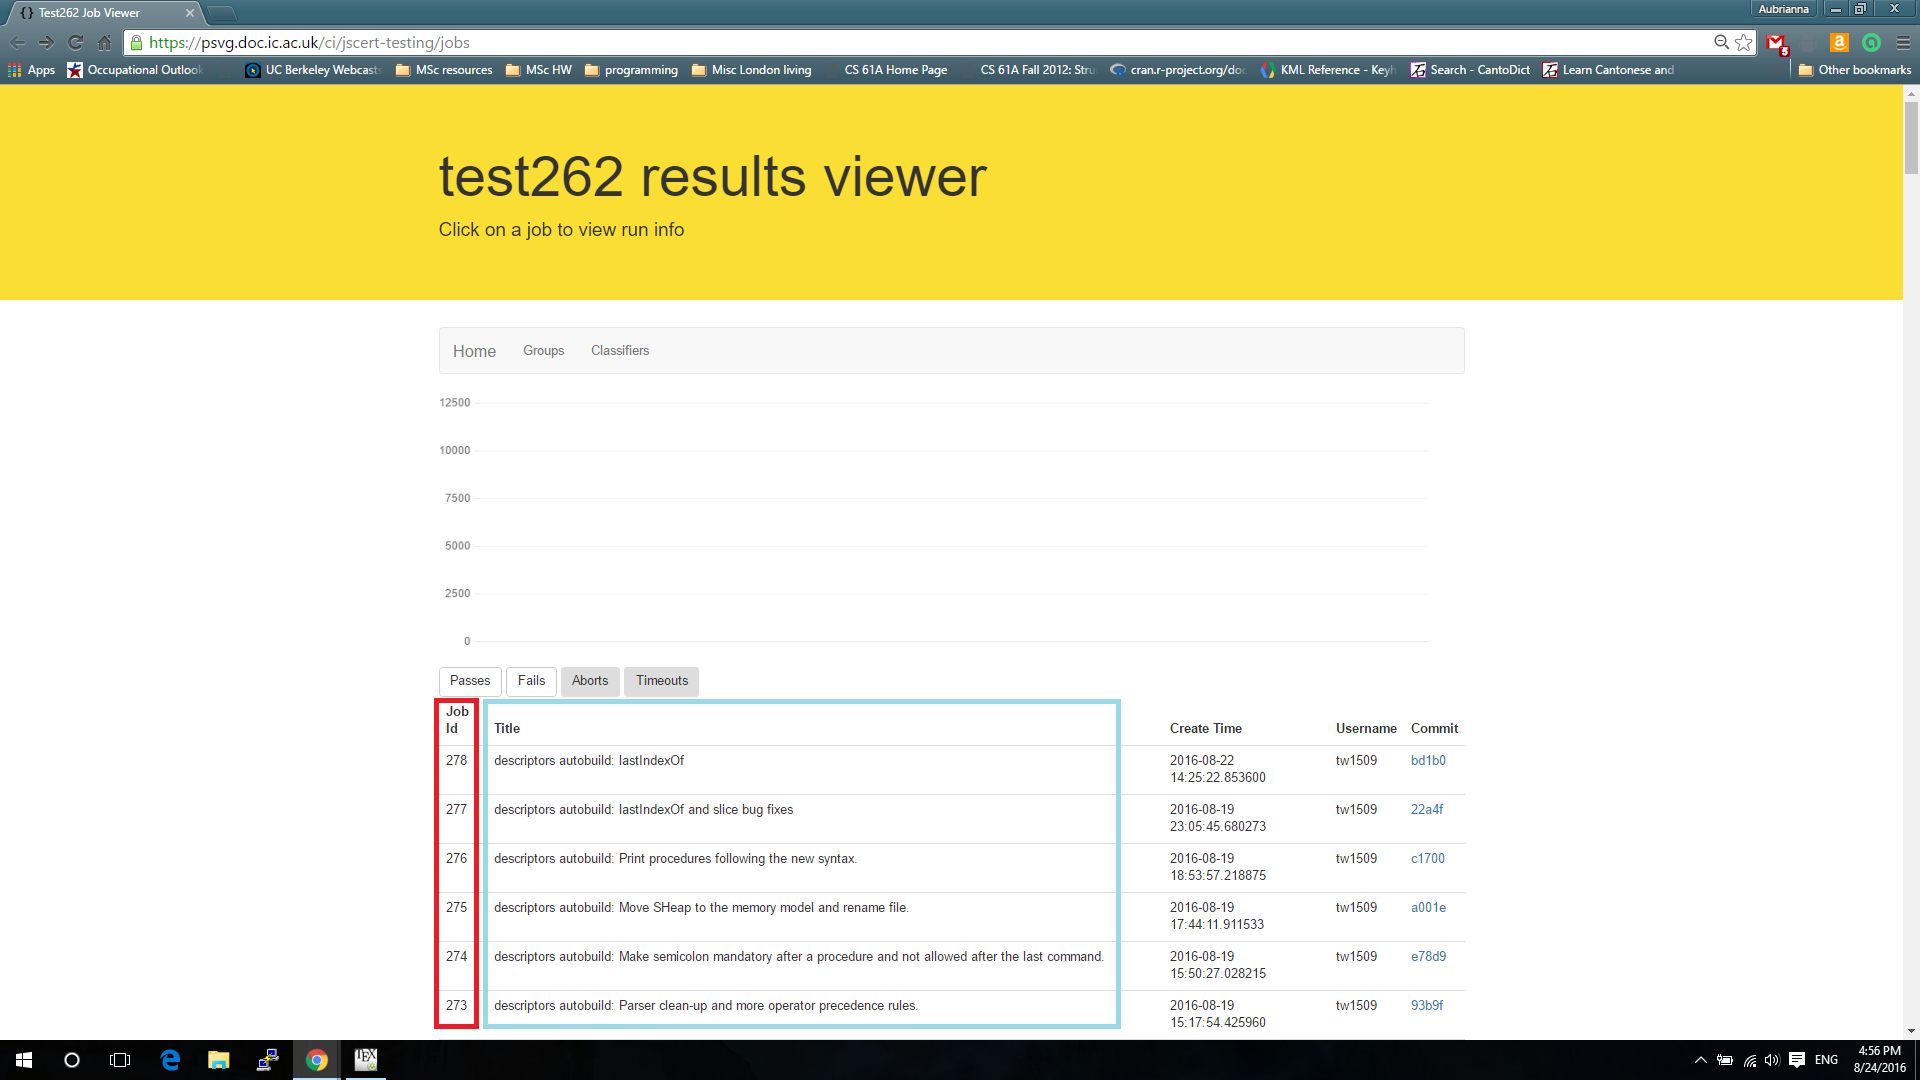
\includegraphics[width=1.0\textwidth]{main_testing_screen_boxed}
\end{figure}

The testing interface can be found at the following web address: https://psvg.doc.ic.ac.uk/ci/jscert-testing/jobs. Figure 11.1 is a screen shot of the landing page of the testing interface. The most important pieces of information on this page are the Job ID, which is boxed in red, and the Title, which is boxed in blue. The Job ID represents the a numbered sequence of Git commits made to the resource-reasoning/JavaScriptVerification project, with the most recent commits at the top of the screen. The Title represents the Git commit message, which ideally includes information about the content of the commit.

\begin{figure}[h!]
  \caption{Individual Job Testing Screen}
  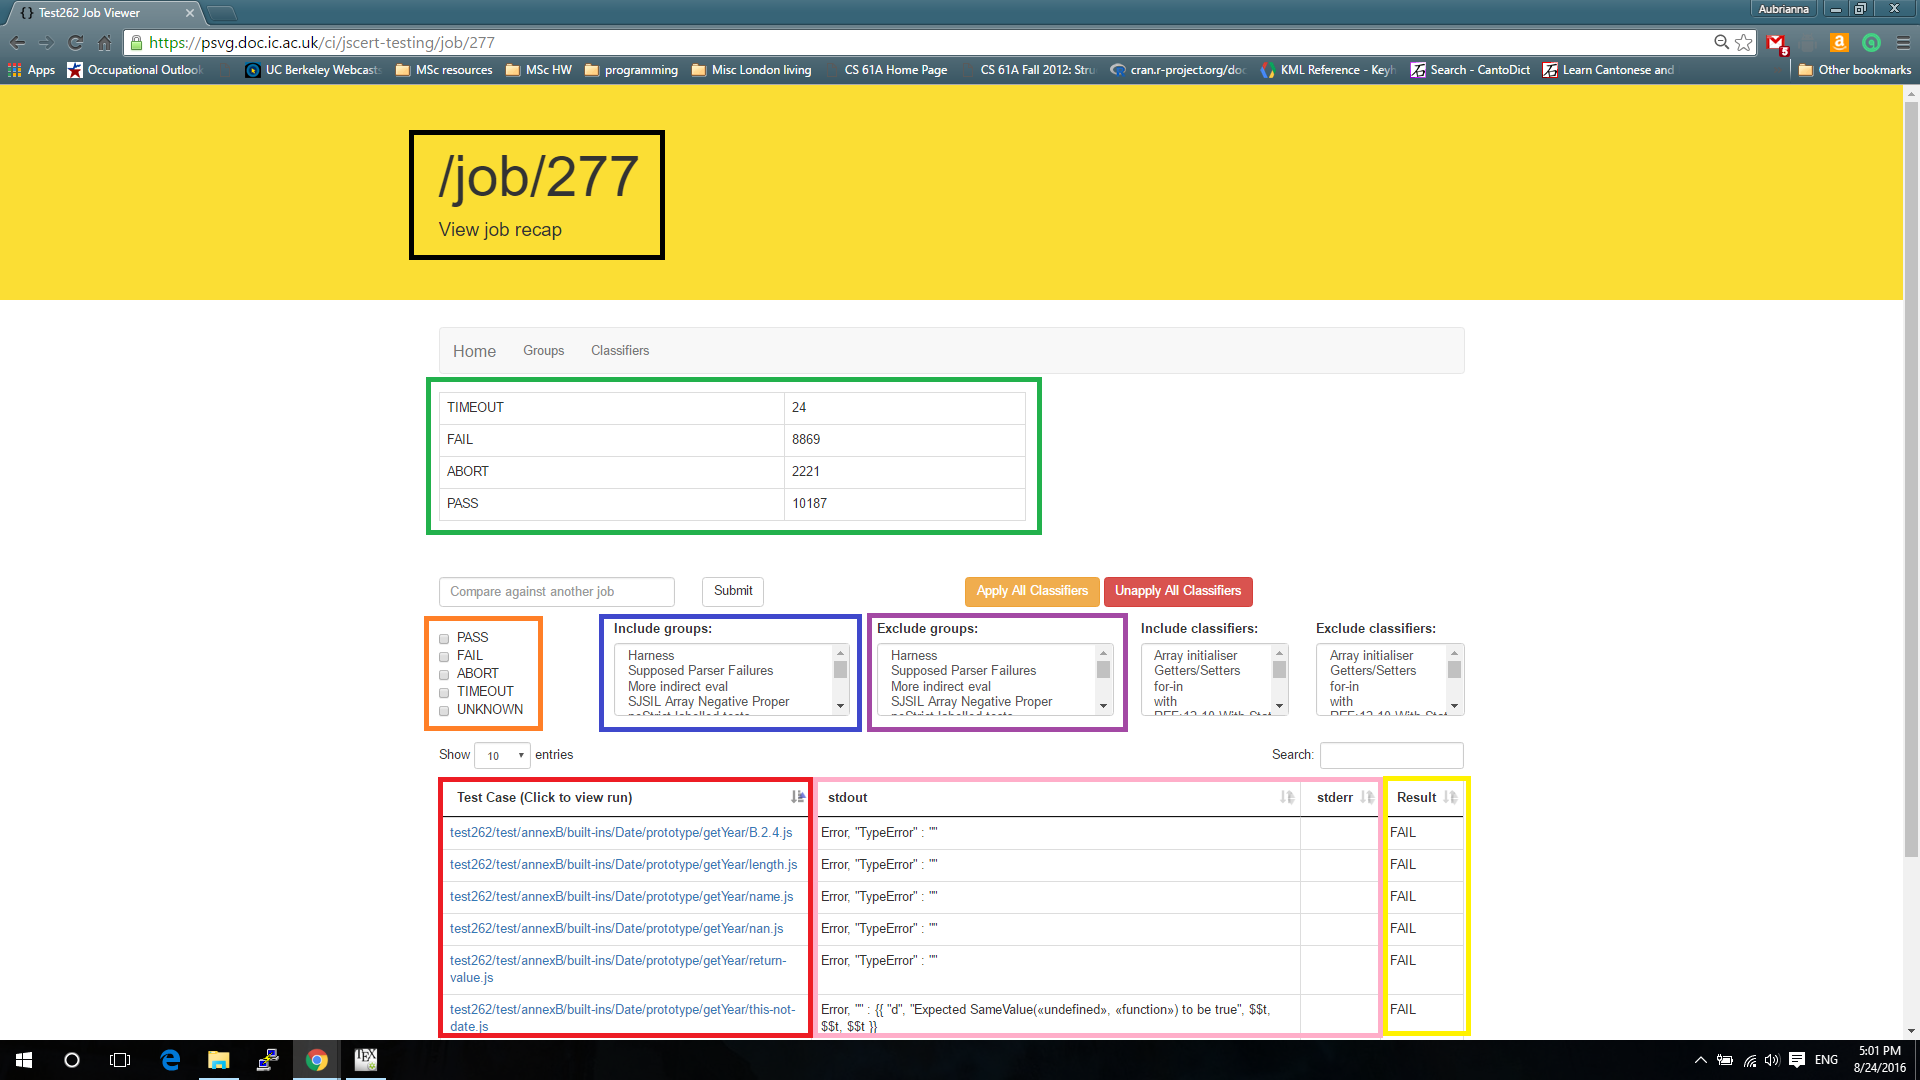
\includegraphics[width=1.0\textwidth]{job_testing_screen_boxed}
\end{figure}

Clicking on either the Job ID or the Title of a commit brings the user to the testing screen for that commit, shown in Figure 11.2. This is the main page for analyzing the tests, and it includes the following pieces of information.

\begin{description}
\item[Job ID] The Job ID is highlighted in black in the header. It shows the user which commit he or she is working with.

\item[Summary Statistics] The summary statistics highlighted in green describes the number of tests in each of the following categories: TIMEOUT, FAIL, ABORT, and PASS. Tests in TIMEOUT are ones that took too long to run, either because the code being tested ran into infinite loops or other such reasons. Tests in FAIL are ones that threw errors into the standard output stream, because the code being tested did not produce the expected results. Tests in ABORT are ones that threw errors into the standard error stream, and they are usually due to JavaScript features that have not yet been implemented in JSIL. Tests in PASSED are ones that produced normal output to the standard output stream with expected results.

\item[Category Checkboxes] The checkboxes highlighted in orange allows the user to filter out tests in one or more specific categories. The first four checkboxes correspond to the categories described previously, and the last checkbox corresponds to the UNKNOWN condition. Tests in UNKNOWN are ones that are still in the queue to be run once a commit is registered on the testing site.

\item[Include Groups] The numerous test cases can be categorized into groups of tests, each targeting a related subset of tests. Most of these groups are created manually, and the creation process will be addressed later. When a group is selected, only the tests belonging to the group will be displayed. Multiple groups can be selected.

\item[Exclude Groups] Groups of tests can be purposefully excluded from the display as well. For example, tests that only pertain to ES6 should be excluded from the analysis because they are outside the scope of this project.

\item[Test Cases] The list of test cases is highlighted in red, and it includes the names of all of the tests the user is looking at. This list includes all of the tests in the test suite by default, and it will be different if the user has included and/or excluded specific groups. Each test is referred to by a test name, which is a hyperlink to a detailed test case page, which will be presented later.

\item[Standard Output and Standard Error] The output of the tests is highlighted in pink, and it includes output to both the standard output stream and the standard error stream. Usually PASSED tests start with "Normal" and the FAILED tests start with "Error" in Stdout, and ABORTED tests start with "Fatal error" in Stderr.

\item[Result] The results are highlighted in yellow, and they show what category the tests fall under.
\end{description} 

\begin{figure}[h!]
  \caption{Test Cases Group}
  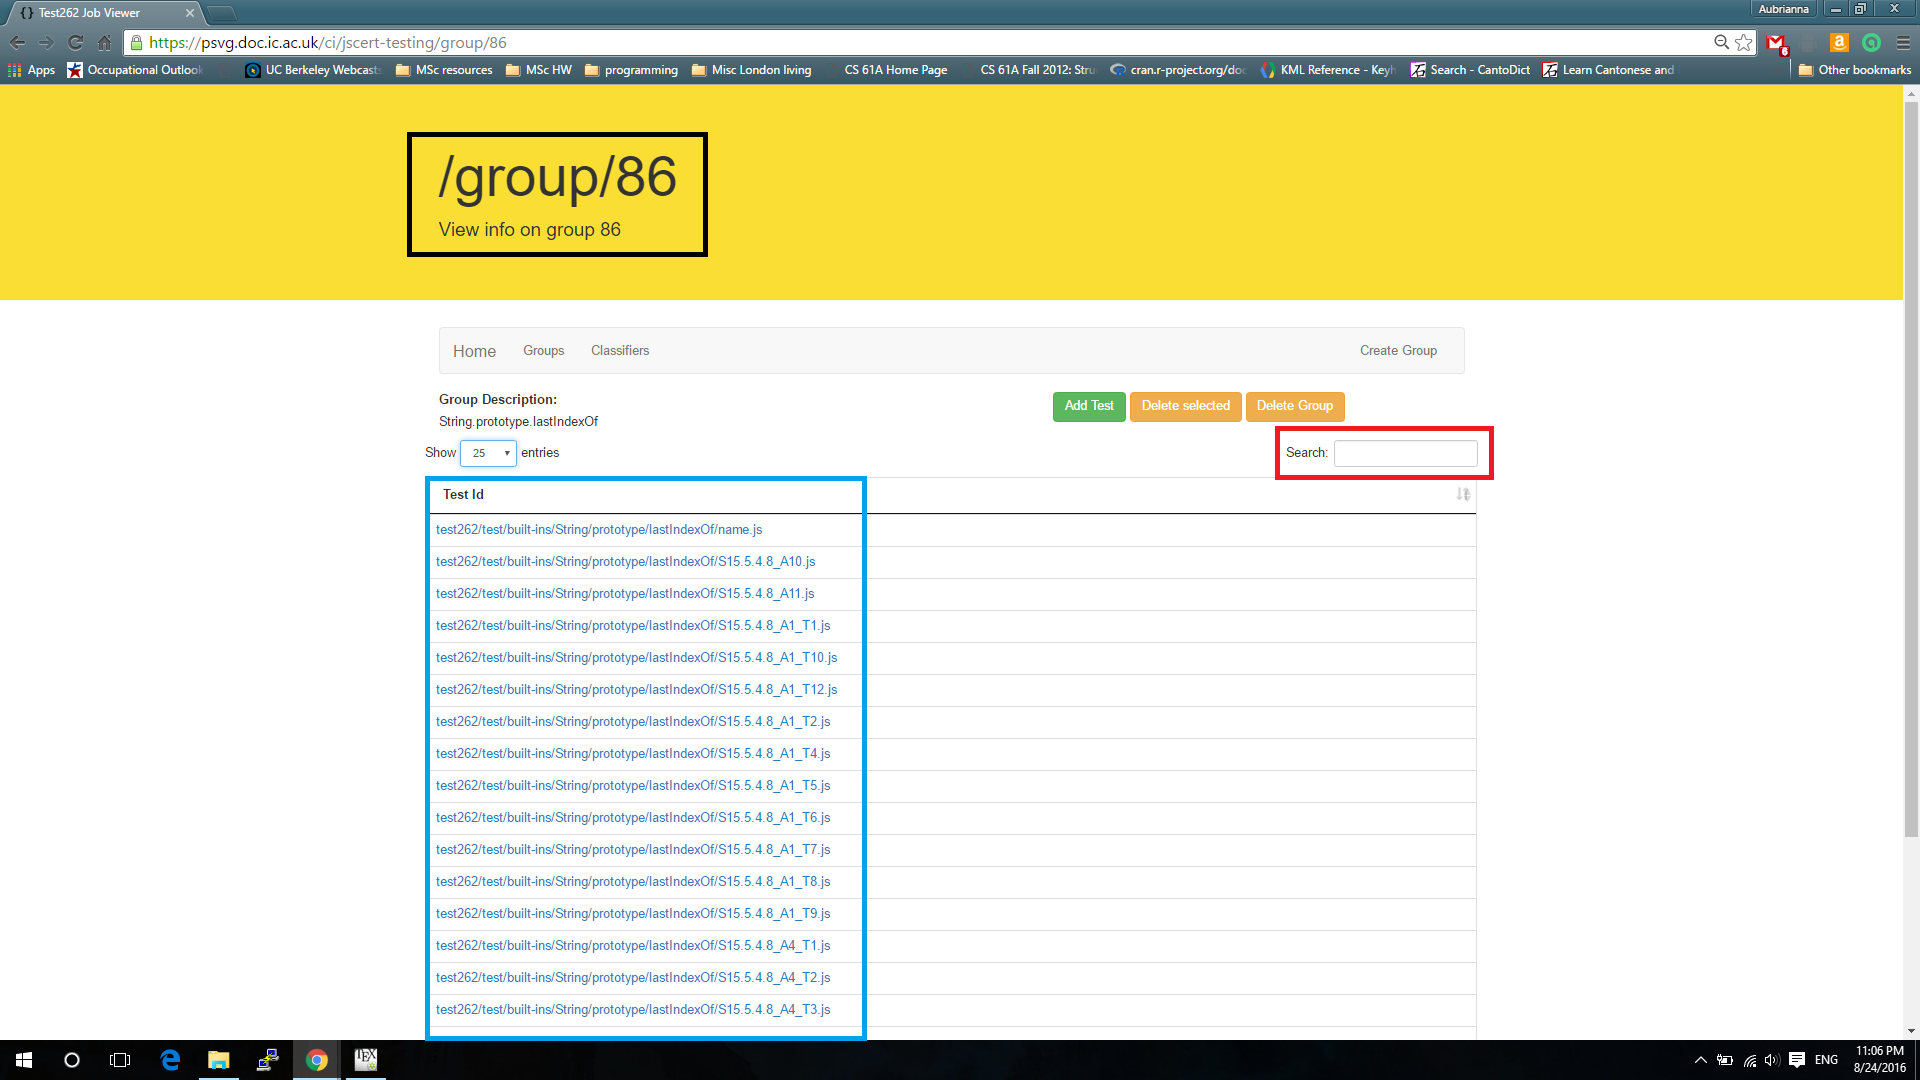
\includegraphics[width=1.0\textwidth]{group_testing_screen_boxed}
\end{figure}

The different test cases groups can be found at https://psvg.doc.ic.ac.uk/ci/jscert-testing/groups/, and from that page, the user can view a specific group like Group 86 presented in Figure 11.3. Highlighted in black in the header is the group number, and highlighted in red is a search box, in which a user can type the name of a test case to see whether a test is already included in the group. The green button for \textbf{Add Test} enables the user to add additional tests into the group. Highlighted in blue is the list of tests belonging to this group. Each test is referred to by a name, and the hyperlink leads the user to a test case history page, which displays the results for this test case for all the recorded test runs. 

\begin{figure}[h!]
  \caption{Test Case Details}
  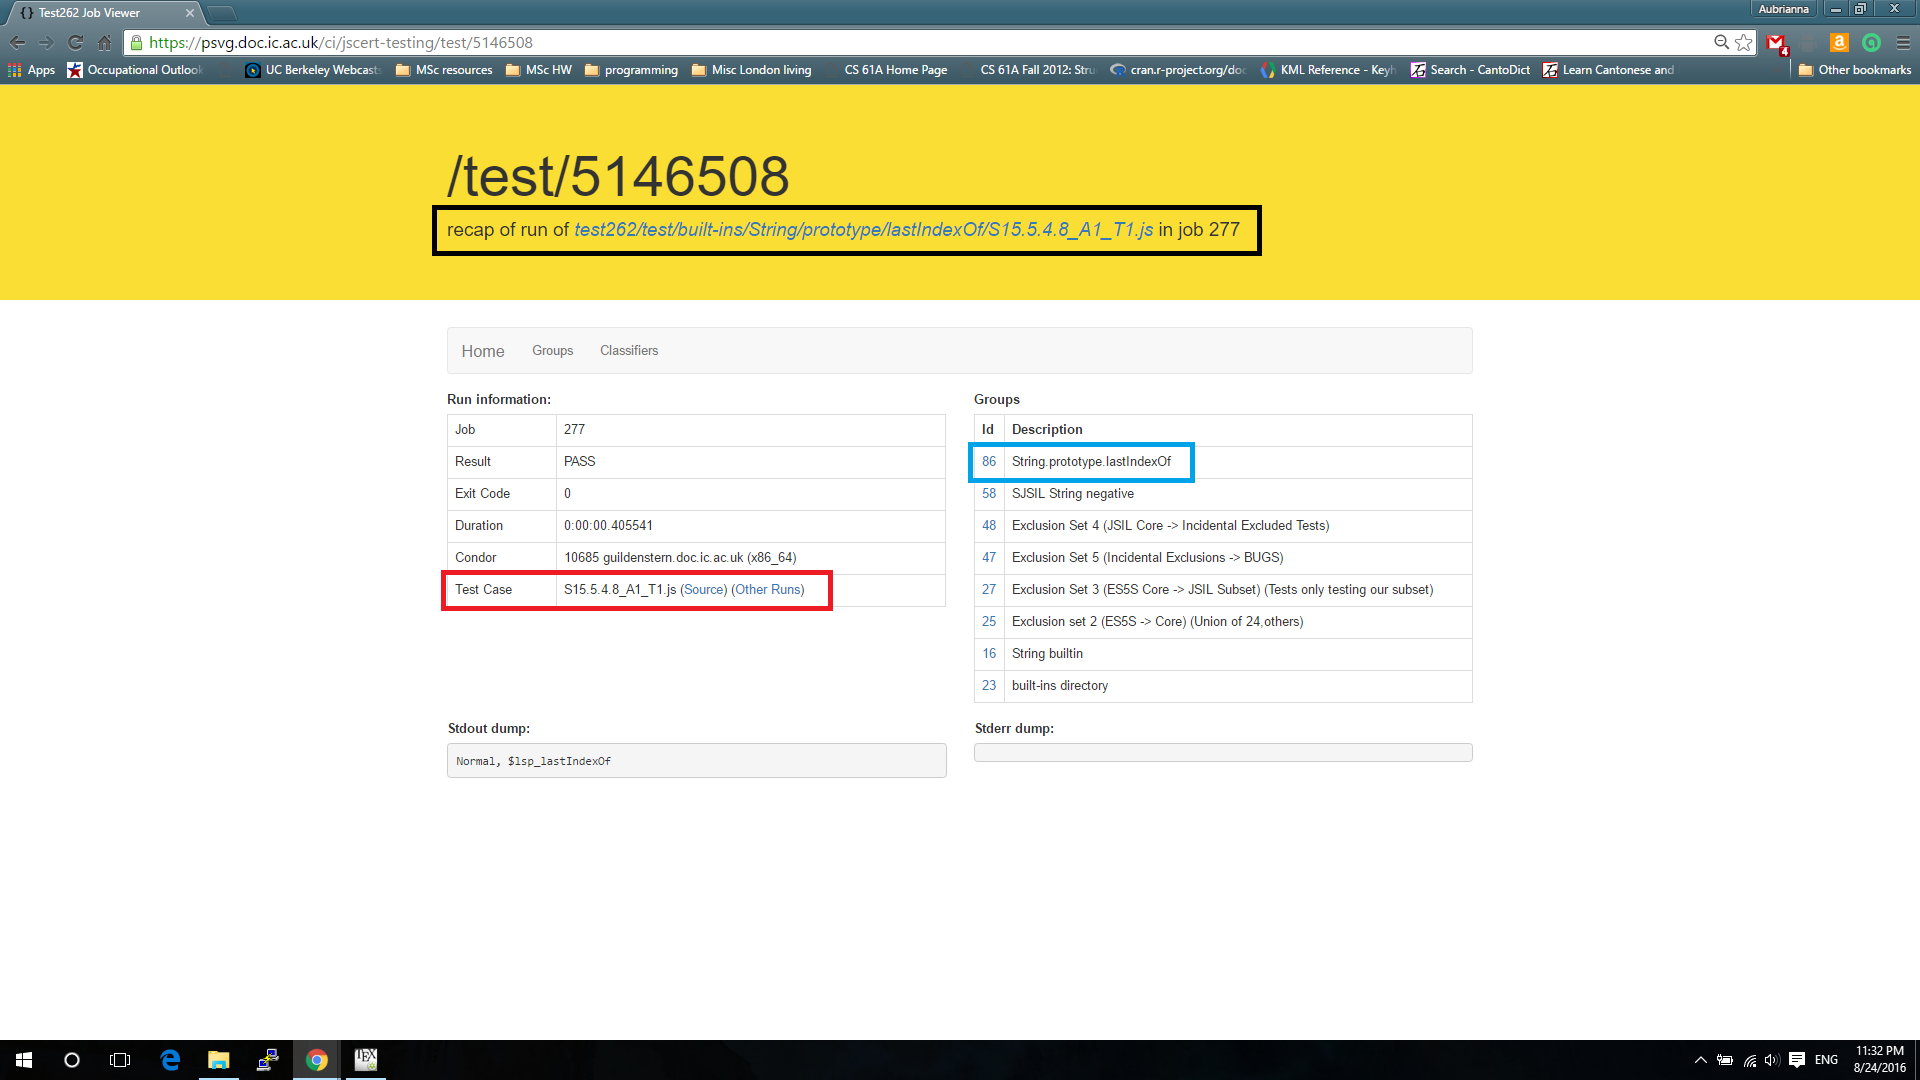
\includegraphics[width=1.0\textwidth]{test_case_testing_screen_boxed}
\end{figure}

If the user clicked the hyperlink on the job page from Figure 11.2, he or she will see a test case details page like the one presented in Figure 11.4. The highlighted black box in the header, as well as the \textbf{Source} text in the red box contain hyperlinks to the source code of the test. The \textbf{Other Runs} text in the red box contains a hyperlink to the test case history page, which is also linked from the test cases group page as mentioned in Figure 11.3. The right hand side shows the group membership of this test, and the group of interest is highlighted in blue.

\begin{figure}[h!]
  \caption{Test Case Source Code}
  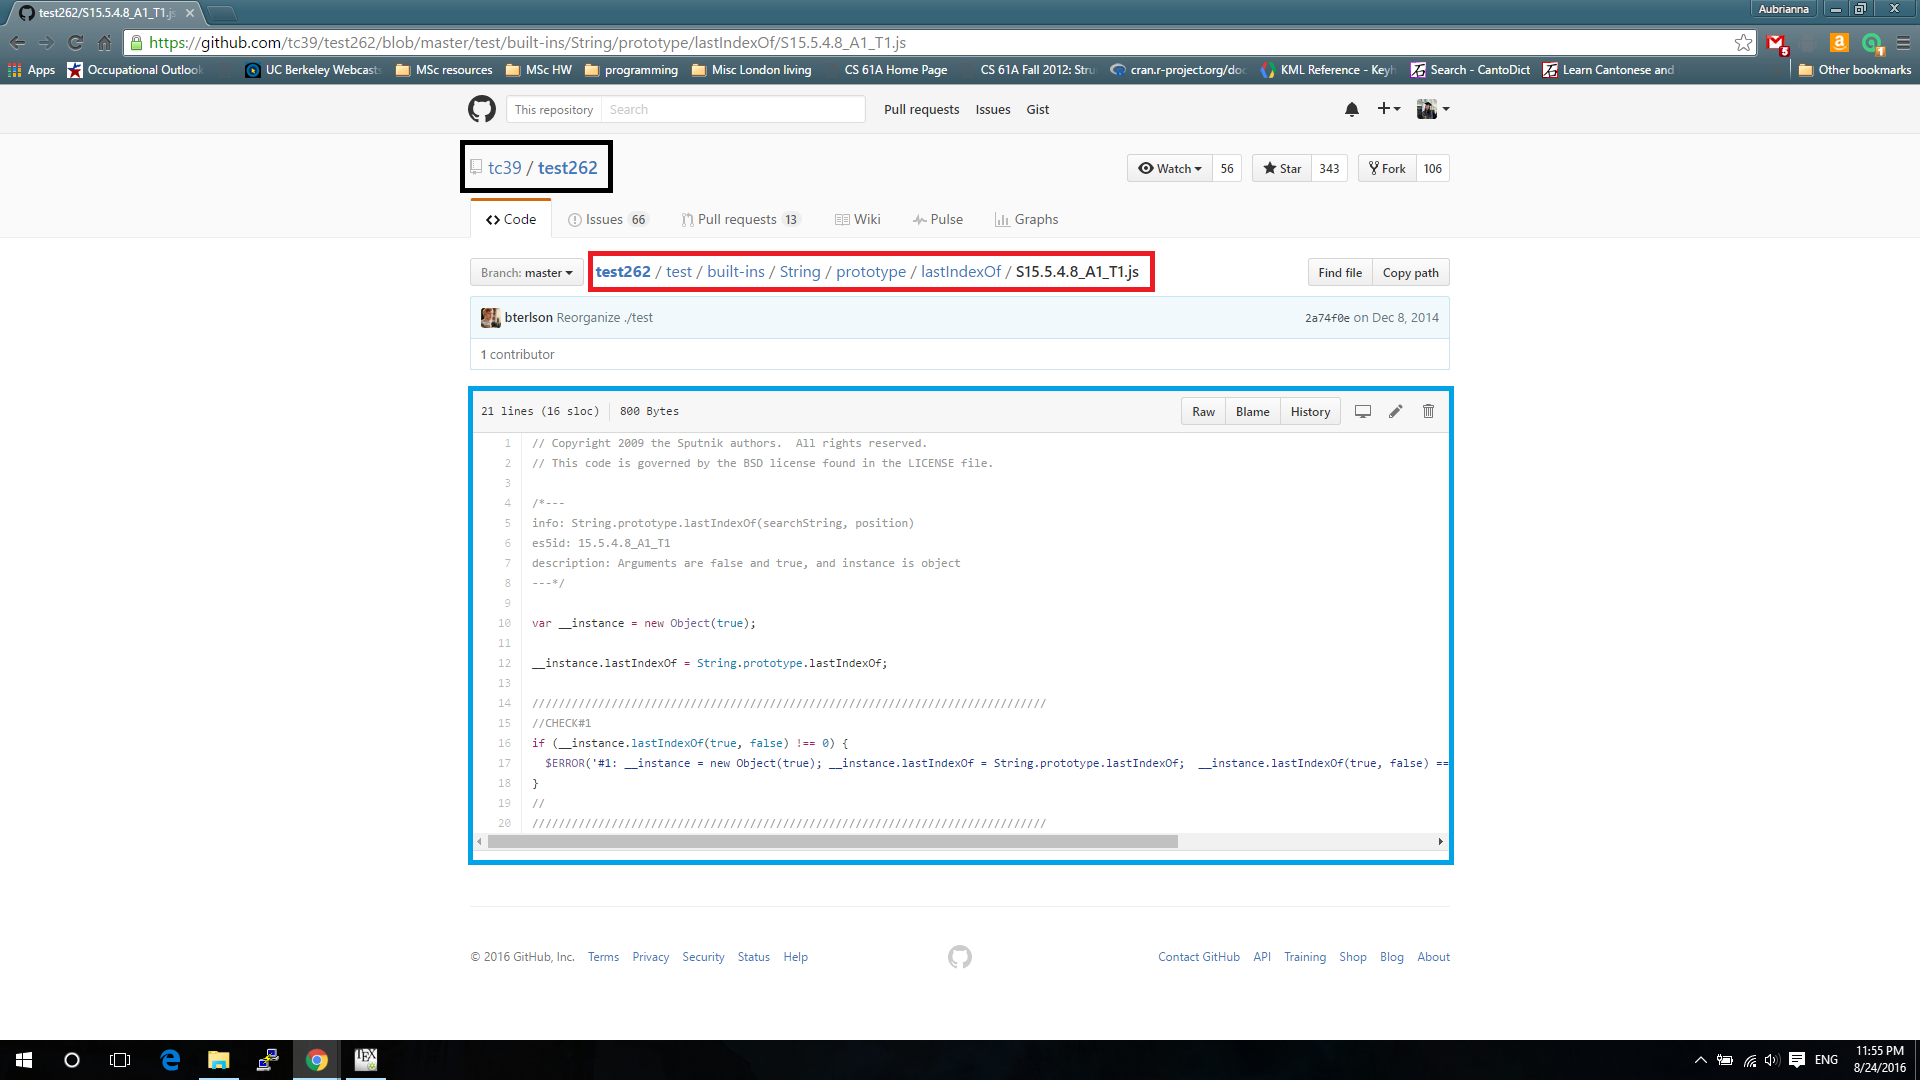
\includegraphics[width=1.0\textwidth]{source_testing_screen_boxed}
\end{figure}

The source code of each test can be viewed on a Github page as shown in Figure 11.5. Highlighted in black on top shows the repository name, which is \textbf{test262}, which belongs to \textbf{tc39}. TC39 refers to Ecma International, Technical Committee 39 - ECMAScript, who are the owner of the \textbf{test262} suite. Highlighted in red is the name of the particular test case, and highlighted in blue is the source code. For tests that produced unexpected behavior, reading the source code to figure out what exactly the test case targets greatly helps in debugging the JSIL program.

%\section{Array Library and Arguments Object}
%\subsection{Array Library}
%%TODO%%???
%\subsection{Arguments Object}

\section{String Library}
As listed in Section~\ref{sec:stringmethods}, six String Library methods were implemented. Tests before implementing any of these methods were analyzed, and five tests have already passed for each method without implementation. Since the tests occur in all methods implemented, the \textbf{METHOD\_NAME} text in the bullet points can be substituted with the actual method names.

\begin{description}
\item[test262/test/built-ins/String/prototype/METHOD\_NAME/S15.5.4.4\_A10.js] This test checks to see if the method's length property is not writable, i.e., its [[writable]] attribute is false. In the implementation, a set of initialization actions have already set this attribute to be false, so this test passed without the actual method implementation.

\item[test262/test/built-ins/String/prototype/METHOD\_NAME/S15.5.4.4\_A11.js] This test checks for the method's length property value. Similarly, this is already determined in the initialization step, and more specifically, the length values for charAt, concat, indexOf, and lastIndexOf are explicitly set to 1, and the length values for slice and substring are set to 2.

\item[test262/test/built-ins/String/prototype/METHOD\_NAME/S15.5.4.4\_A6.js] This test checks to see that the method does not have a prototype property.

\item[test262/test/built-ins/String/prototype/METHOD\_NAME/S15.5.4.4\_A7.js] This test checks to see that the method cannot be used as a constructor to create a new object. When all of these methods are created in the initialization step, their \textbf{construct} property is set to \textbf{empty}, so this test passed without actual method implementation.

\item[test262/test/built-ins/String/prototype/METHOD\_NAME/S15.5.4.4\_A8.js] This test checks to see if the method's length property is not enumerable, i.e., its [[enumerable]] attribute is false. The initialization step also sets this attribute to false, so this test passed before the actual method was implemented.
\end{description}

In addition, for each method there are two tests that have failed before any implementation, because the first is a new ES6 feature, and the second represents a change in program logic from ES5 to ES6.

\begin{description}
\item[test262/test/built-ins/String/prototype/METHOD\_NAME/name.js] In ES6, built-in function objects that are not anonymous functions all have a \textbf{name} property, whose [[value]] attribute is a String value. Its [[writable]] and [[enumerable]] attributes are false by default, and its [[configurable]] attribute is true by default.

\item[test262/test/built-ins/String/prototype/METHOD\_NAME/S15.5.4.4\_A9.js] This test checks to see if the method's length property has the DontDelete attribute. In ES6, String methods' length property do not have the DontDelete attribute, and therefore can be deleted using the \textbf{delete} keyword. In ES5, however, since the length property in each method is not configurable, it cannot be deleted.
\end{description}

\begin{itemize}
\item String.prototype.charAt(pos) \\
In addition to the tests that have already passed and failed, there were 18 tests that were aborted for this method prior to any implementation, for a total of 25 tests. After completing implementation for charAt and rerunning the tests, there were still three ABORTED tests because they utilized the String.prototype.substring method to test charAt, but substring had not been implemented.
\begin{itemize}
\item test262/test/built-ins/String/prototype/charAt/S15.5.4.4\_A4\_T1.js
\item test262/test/built-ins/String/prototype/charAt/S15.5.4.4\_A4\_T2.js
\item test262/test/built-ins/String/prototype/charAt/S15.5.4.4\_A4\_T3.js
\end{itemize}
After completing the substring method, these three tests passed as well. Excluding the nonrelevant tests, all 23 test cases for charAt have passed.
\begin{table}[ht!]
\centering
\begin{subtable}{0.5\textwidth}
\centering
\begin{tabular}{|p{3cm}|p{2cm}|} \hline
\textbf{Test Category} & \textbf{Count} \\ \hline
Pass & 5 \\
Fail & 2 \\
Abort & 18 \\
Timeout & 0 \\
Total & 25 \\ \hline
\end{tabular}
\caption{Before Implementation}
\end{subtable}%
\begin{subtable}{0.5\textwidth}
\centering
\begin{tabular}{|p{3cm}|p{2cm}|} \hline
\textbf{Test Category} & \textbf{Count} \\ \hline
Pass & 23 \\
Fail & 0 \\
Abort & 0 \\
Timeout & 0 \\
Total & 23 \\ \hline
\end{tabular}
\caption{After two rounds of implementations}
\end{subtable}
\caption{String.prototype.charAt(pos)}
\end{table}

\item String.prototype.concat( [ string1 [, string2 [, ...]]] ) \\
The concat method was straightforward. There were 13 ABORTED tests prior to any implementation, and all 13 passed after the first round of coding. Excluding the two nonrelevant tests, all 18 test cases passed for concat.
\begin{table}[ht!]
\centering
\begin{subtable}{0.5\textwidth}
\centering
\begin{tabular}{|p{3cm}|p{2cm}|} \hline
\textbf{Test Category} & \textbf{Count} \\ \hline
Pass & 5 \\
Fail & 2 \\
Abort & 13 \\
Timeout & 0 \\
Total & 20 \\ \hline
\end{tabular}
\caption{Before Implementation}
\end{subtable}%
\begin{subtable}{0.5\textwidth}
\centering
\begin{tabular}{|p{3cm}|p{2cm}|} \hline
\textbf{Test Category} & \textbf{Count} \\ \hline
Pass & 18 \\
Fail & 0 \\
Abort & 0 \\
Timeout & 0 \\
Total & 18 \\ \hline
\end{tabular}
\caption{After Implementation}
\end{subtable}
\caption{String.prototype.concat( [ string1 [, string2 [, ...]]] )}
\end{table}

\item String.prototype.indexOf(searchString, position) \\
In addition to the five PASSED tests and two FAILED tests, indexOf had an additional test in the PASSED category prior to any method implementation.
\begin{itemize}
\item test262/test/built-ins/String/prototype/indexOf/S15.5.4.7\_A1\_T12.js \\
This test checks to see whether an Array Object that included Strings as elements would be indexed correctly. As the Array Library had already been implemented, and it had the ability to hold any type of JavaScript Object in an Array, this test passed without the String method implementation.
\end{itemize}
After the first round of coding, an additional 21 test cases passed, but 7 tests were still in the ABORTED category, because they required additional methods from the Date and String Libraries that are outside the scope of this project. More specifically, one test required the Date.prototype.getTimezoneOffset method, and six tests required the String.fromCharCode method. Excluding the two nonrelevant tests, there were a total of 27 PASSED tests and 7 ABORTED tests for a total of 34 test cases.
\begin{table}[ht!]
\centering
\begin{subtable}{0.5\textwidth}
\centering
\begin{tabular}{|p{3cm}|p{2cm}|} \hline
\textbf{Test Category} & \textbf{Count} \\ \hline
Pass & 6 \\
Fail & 2 \\
Abort & 28 \\
Timeout & 0 \\
Total & 36 \\ \hline
\end{tabular}
\caption{Before Implementation}
\end{subtable}%
\begin{subtable}{0.5\textwidth}
\centering
\begin{tabular}{|p{3cm}|p{2cm}|} \hline
\textbf{Test Category} & \textbf{Count} \\ \hline
Pass & 27 \\
Fail & 0 \\
Abort & 7 \\
Timeout & 0 \\
Total & 34 \\ \hline
\end{tabular}
\caption{After Implementation}
\end{subtable}
\caption{String.prototype.indexOf(searchString, position)}
\end{table}

\item String.prototype.lastIndexOf(searchString, position) \\
Similar to indexOf, lastIndexOf also had six passing tests before any method implementation, and the test case below also tested for whether an element in an Array Object can be correctly identified from the lastIndexOf operation.
\begin{itemize}
\item test262/test/built-ins/String/prototype/lastIndexOf/S15.5.4.8\_A1\_T12.js
\end{itemize}
After the first round of coding, 10 additional tests passed, and the 4 tests below failed. 
\begin{itemize}
\item test262/test/built-ins/String/prototype/lastIndexOf/S15.5.4.8\_A1\_T1.js \\
This test creates an Object with the boolean value \textbf{true}, and tries to find the index of \textbf{true} within the Object instance, provided the Object's lastIndexOf method is the same as String's lastIndexOf method. Upon analyzing the test source code and the JSIL implementation, it was discovered that the JSIL logic was incorrectly implemented. The first version of the JSIL lastIndexOf could not handle cases where the searchString was the same length or larger than the String Object performing the method.
\item test262/test/built-ins/String/prototype/lastIndexOf/S15.5.4.8\_A1\_T2.js \\
This test creates a Boolean Object, and sets the Object's lastIndexOf method to be that of String's. Because the default value for a Boolean Object is \textbf{false}, when the lastIndexOf method is called on the Boolean Object, passing in inputs that essentially reduce to \textbf{false} should find a match at the beginning of the string. This case is similar to the previous one, and was fixed by handling searchString inputs of the same size as the String Object itself.
\item test262/test/built-ins/String/prototype/lastIndexOf/S15.5.4.8\_A1\_T10.js \\
This test checks to see if looking for a searchString from a position that is not a number, i.e., \textbf{NaN}, would produce the correct results. The initial JSIL implementation incorrectly disregarded the step to check whether the position parameter is not a number, whereas the correct implementation should convert \textbf{NaN} to positive infinity.
\item test262/test/built-ins/String/prototype/lastIndexOf/S15.5.4.8\_A4\_T3.js \\
This test creates a searchString and an empty Object as the index position. Upon inputting these parameters into a String value calling its lastIndexOf method, the empty Object should be converted to \textbf{NaN}, and the rest of the logic is as presented for the previous test case.
\end{itemize}
Two rounds of bug-fixing and re-testing resulted in their passing. In the end, excluding nonrelevant test cases, all 20 test cases passed.
\begin{table}[ht!]
\centering
\begin{subtable}{0.5\textwidth}
\centering
\begin{tabular}{|p{3cm}|p{2cm}|} \hline
\textbf{Test Category} & \textbf{Count} \\ \hline
Pass & 6 \\
Fail & 2 \\
Abort & 14 \\
Timeout & 0 \\
Total & 22 \\ \hline
\end{tabular}
\caption{Before Implementation}
\end{subtable}%
\begin{subtable}{0.5\textwidth}
\centering
\begin{tabular}{|p{3cm}|p{2cm}|} \hline
\textbf{Test Category} & \textbf{Count} \\ \hline
Pass & 20 \\
Fail & 0 \\
Abort & 0 \\
Timeout & 0 \\
Total & 20 \\ \hline
\end{tabular}
\caption{After two rounds of implementations}
\end{subtable}
\caption{String.prototype.lastIndexOf(searchString, position)}
\end{table}

\item String.prototype.slice(start, end) \\
Before any method implementation, there were five PASSED tests, two FAILED tests, and 27 ABORTED tests. After the first round of coding, 14 additional tests passed, but 13 were still aborted. 
\begin{itemize}
\item test262/test/built-ins/String/prototype/slice/S15.5.4.13\_A1\_T5.js \\
This test sets the Function prototype slice method to the String prototype slice method, but since the Function Object constructor had not been implemented, it was impossible to run this test.
\item test262/test/built-ins/String/prototype/slice/S15.5.4.13\_A1\_T14.js \\
This test passes an empty Function Object into the slice method of a String value, and this empty Object should be converted into \textbf{NaN}. The initial JSIL implementation only took into account cases where the start parameter can be successfully converted to an integer value, thus it failed when trying to index on \textbf{NaN}. Changes to the code was made to set the start value to be the beginning of the String if the start input cannot be successfully converted to an integer.
\item test262/test/built-ins/String/prototype/slice/S15.5.4.13\_A1\_T15.js \\
This test creates a Number Object, sets its prototype.slice method to be that of String's prototype.slice, and calls the method with no inputs. Similar to the previous test case, the initial JSIL implementation failed because an empty argument cannot be transformed into an integer.
\item test262/test/built-ins/String/prototype/slice/S15.5.4.13\_A1\_T6.js \\
This test attempts to pass \textbf{Undefined} into the slice method as the start input, and was similarly fixed by setting a default start value.
\item test262/test/built-ins/String/prototype/slice/S15.5.4.13\_A2\_T1.js \\
This test creates a String Object, slices the entire String, and checks to see if the \textbf{typeof} value for this Object is the value "string". The test calls the slice method with no inputs, so the start value should be taken as the beginning of the String by default, and this test was similarly fixed by setting a default start.
\end{itemize}

The following test cases were aborted because of a mistake of variable name referencing in the JSIL implementation. JSIL has an internal indexing mechanism for strings, which only takes positive integers as input for indices, but the initial JSIL implementation incorrectly used the direct input value, rather than the calculated value, as the string index. In addition, when the start and end inputs vary by more than one index value, the start index is incremented to get the consecutive string characters until the end index is reached. In the first JSIL implementation, however, an incorrect start index was incremented.
\begin{itemize}
\item test262/test/built-ins/String/prototype/slice/S15.5.4.13\_A1\_T1.js \\
This test inputs the boolean values false and true into the slice method. When indexing the string in JSIL, the initial JSIL function used the boolean value, rather than an integer converted from this boolean. Hence JSIL was unable to provide the string character at the given start index.
\item test262/test/built-ins/String/prototype/slice/S15.5.4.13\_A1\_T2.js \\
This test uses a function object that returns the boolean value true as the start value given to the slice method, and thus JSIL was unable to correctly index the string.
\item test262/test/built-ins/String/prototype/slice/S15.5.4.13\_A1\_T8.js \\
This test used a negative integer as the start input, and JSIL requires nonnegative indices for strings.
\item test262/test/built-ins/String/prototype/slice/S15.5.4.13\_A2\_T2.js \\
This test uses \textbf{NaN} as the start input, which is not an integer and therefore could not be used as a string index in JSIL.
\item test262/test/built-ins/String/prototype/slice/S15.5.4.13\_A3\_T3.js \\
This test uses negative infinity as the start input, which is not an integer and therefore could not be used as a string index in JSIL.
\item test262/test/built-ins/String/prototype/slice/S15.5.4.13\_A1\_T4.js \\
This test uses \textbf{null} as the start input, which is not an integer and therefore could not be used as a string index in JSIL.
\item test262/test/built-ins/String/prototype/slice/S15.5.4.13\_A1\_T7.js \\
This test uses a string value as the start input, therefore it could not be used as a string index in JSIL.
\item test262/test/built-ins/String/prototype/slice/S15.5.4.13\_A1\_T10.js \\
This test uses a Function Object as the start input, therefore it could not be used as a string index in JSIL.
\end{itemize}

After fixing the above-mentioned issues, only one test remained in the ABORTED state, but since its passing requires the Function Object constructor, it is out of the scope of this project and is therefore left unimplemented. Otherwise, there remain 31 relevant test cases, all of which were in PASSED.
\begin{table}[ht!]
\centering
\begin{subtable}{0.5\textwidth}
\centering
\begin{tabular}{|p{3cm}|p{2cm}|} \hline
\textbf{Test Category} & \textbf{Count} \\ \hline
Pass & 5 \\
Fail & 2 \\
Abort & 27 \\
Timeout & 0 \\
Total & 34 \\ \hline
\end{tabular}
\caption{Before Implementation}
\end{subtable}%
\begin{subtable}{0.5\textwidth}
\centering
\begin{tabular}{|p{3cm}|p{2cm}|} \hline
\textbf{Test Category} & \textbf{Count} \\ \hline
Pass & 31 \\
Fail & 0 \\
Abort & 1 \\
Timeout & 0 \\
Total & 32 \\ \hline
\end{tabular}
\caption{After two rounds of implementations}
\end{subtable}
\caption{String.prototype.slice(start, end)}
\end{table}

\item String.prototype.substring(start, end) \\
The substring method was relatively straightforward as well. There were 35 ABORTED tests before method implementation, and after the first round of coding, one test remained ABORTED. 
\begin{itemize}
\item test262/test/built-ins/String/prototype/substring/S15.5.4.15\_A1\_T5.js \\
This test sets the Function prototype substring method to the String prototype substring method, but since the Function Object constructor had not been implemented, it was impossible to run this test.
\end{itemize}
Excluding the nonrelevant tests, there were a total of 40 test cases, of which 39 passed, and one aborted.
\begin{table}[ht!]
\centering
\begin{subtable}{0.5\textwidth}
\centering
\begin{tabular}{|p{3cm}|p{2cm}|} \hline
\textbf{Test Category} & \textbf{Count} \\ \hline
Pass & 5 \\
Fail & 2 \\
Abort & 35 \\
Timeout & 0 \\
Total & 42 \\ \hline
\end{tabular}
\caption{Before Implementation}
\end{subtable}%
\begin{subtable}{0.5\textwidth}
\centering
\begin{tabular}{|p{3cm}|p{2cm}|} \hline
\textbf{Test Category} & \textbf{Count} \\ \hline
Pass & 39 \\
Fail & 0 \\
Abort & 1 \\
Timeout & 0 \\
Total & 40 \\ \hline
\end{tabular}
\caption{After Implementation}
\end{subtable}
\caption{String.prototype.substring(start, end)}
\end{table}

\end{itemize}






%%%%%%%%%%%%%%%%%%%%%%%%%%%%%%%%%%%%
\chapter{Conclusion}


%% bibliography
\bibliographystyle{plain}
\bibliography{refs}

\end{document}
